\documentclass[12pt,a4paper]{report}

%\includeonly{cover/cimlap, chapters/1_introduction}

\usepackage{styles/dolgozat}

% programkód beillesztéséhez
\usepackage{listings}
% listing float neve
\renewcommand{\lstlistingname}{Programkód}
%\renewcommand{\lstlistlistingname}{Programkódok listája}
%saját listings style-ok, és a style-t használó parancsok definíciói
\usepackage{styles/cpp}
\usepackage{styles/python}
%\usepackage{styles/java}
%\usepackage{styles/rust}

%% egyéb csomagok betöltése itt, vagy a dolgozat.sty fájlban

\usepackage{hyperref}
% cleveref csomag és beállításai -- az egyetlen, amit a hyperref után kell betölteni!
\usepackage{styles/refs}
\usepackage{styles/sharp}

\begin{document}

\pagestyle{empty}
\pagenumbering{gobble}

\begin{titlepage}
\centering
% A Miskolci Egyetem címere
\vspace*{2cm}
\huge\textsc{\textbf{Szakdolgozat}}\\[1cm]
%\vspace*{1cm}

\includegraphics[width=4.8cm, height=4cm,keepaspectratio]{images/me_logo.png}\\
\textbf{\textsc{Miskolci Egyetem}}

\vspace*{2cm}

% A szakdolgozat címe, akár több sorban is
{\LARGE\textbf{Komplex stratégiai kártyajáték megtervezése és megvalósítása}}

\vspace*{2cm}
% A hallgató neve, évfolyam, szak(ok), a konzulens(ek) neve
\large
\textbf{Készítette:}\\[0.8ex]
Kriston Ádám\\[0.8ex]
Programtervező informatikus

\vspace*{0.5cm}
\textbf{Témavezető:}\\[0.8ex]
Gégény Dávid

\vfill

% Keltezés: Hely, év
\large
\textbf{\textsc{Miskolc, 2024}}

\end{titlepage}
%Feladatkiiras
\noindent
\textsc{\textbf{Miskolci Egyetem}}\\
Gépészmérnöki és Informatikai Kar\\
Alkalmazott Matematikai Intézeti Tanszék\hspace*{4cm}\hfil \textbf{Szám:}

\vspace{0.5cm}
\begin{center}
\large\textsc{\textbf{Szakdolgozat Feladat}}
\end{center}
\vspace{0.5cm}

Kriston Ádám (SYQ7E2) programtervező informatikus jelölt részére.

\bigskip
\noindent\textbf{A szakdolgozat tárgyköre:} Játék készítés, Kártya játék, Unity, C\#

\bigskip
\noindent\textbf{A szakdolgozat címe:} Komplex stratégiai kártyajáték megtervezése és megvalósítása

\bigskip
\noindent\textbf{A feladat részletezése:}

\medskip

A szakdolgozat egy 2 személyes, komplex játékmechanikával rendelkező kártyajáték megtervezését, annak számítógépes implementációját mutatja be.

Főként a szerepjátékokban elterjedt elemkészletet, megoldásokat használja. A játék 8 alap karakterosztályra építkezik, melyek a játék szempontjából sajátos előnyökkel és hátrányokkal rendelkeznek.

A dolgozat céljai között egyaránt szerepel a játék szabályrendszerének kidolgozása, paraméterek hangolása, a játék megvalósítása, beleértve a gépi ellenfelet. Az alkalmazás elkészítése C\# programozási nyelven történik.

\vfill

\noindent\textbf{Témavezető:} Témavezető neve (beosztása)

% \noindent\textbf{Konzulens(ek):} (akkor kötelezõ, ha a témavezetõ nem valamelyik matematikai tanszékrõl való; de persze lehet egyébként is)\newline

\bigskip
\noindent\textbf{A feladat kiadásának ideje:}

%\noindent\textbf{A feladat beadásának határideje:}

\vspace{1.5cm}

\hfill\makebox[6cm]{\dotfill}

\hfill\makebox[6cm]{szakfelelős}

\clearpage

\vspace*{1cm}  
\begin{center}
\large\textsc{\textbf{Eredetiségi Nyilatkozat}}
\end{center}
\vspace*{2cm}  

Alulírott \textbf{Szakdolgozó Neve}; Neptun-kód: \texttt{N3P7UN} a Miskolci Egyetem Gépészmérnöki és Informatikai Karának végzős Programtervező informatikus szakos hallgatója ezennel büntetőjogi és fegyelmi felelősségem tudatában nyilatkozom és aláírásommal igazolom, hogy \textit{Szakdolgozat Címe}
című szakdolgozatom saját, önálló munkám; az abban hivatkozott szakirodalom
felhasználása a forráskezelés szabályai szerint történt.

\medskip
Tudomásul veszem, hogy szakdolgozat esetén plágiumnak számít:
\begin{itemize}
\item szószerinti idézet közlése idézőjel és hivatkozás megjelölése nélkül;
\item tartalmi idézet hivatkozás megjelölése nélkül;
\item más publikált gondolatainak saját gondolatként való feltüntetése.
\end{itemize}

Alulírott kijelentem, hogy a plágium fogalmát megismertem, és tudomásul veszem, hogy
plágium esetén szakdolgozatom visszautasításra kerül.

\vspace*{3cm}

\noindent Miskolc, \makebox[2cm]{\dotfill}. év \makebox[2cm]{\dotfill}. hó \makebox[2cm]{\dotfill}. nap

\vspace*{3cm}

\hfill\makebox[6cm]{\dotfill}

\hfill\makebox[6cm]{Hallgató}



\clearpage

\newcommand{\ki}{témavezető(k)}
\newsavebox{\alairas}
\begin{lrbox}{\alairas}
\begin{tabular}{c@{\hspace{2cm}}c}
\makebox[4cm]{\dotfill} & \makebox[5cm]{\dotfill} \\
dátum & \ki \\
\end{tabular}
\end{lrbox}
\newcommand{\dotline}{\makebox[5cm]{\dotfill}}
\newcommand{\shortdotline}{\makebox[3.5cm]{\dotfill}}

\noindent 1.
\begin{tabular}[t]{cl}
\multirow{2}{*}{A szakdolgozat feladat módosítása}
&szükséges (módosítás külön lapon) \\
& nem szükséges\\[1ex]
\end{tabular}

\begin{center}
\usebox{\alairas}
\end{center}

\smallskip

\noindent 2. A feladat kidolgozását ellenőriztem:

\begin{center}
\begin{tabular}{c@{\hspace*{2cm}}c}
témavezető (dátum, aláírás): & konzulens (dátum, aláírás):\\
\dotline & \dotline \\
\dotline & \dotline \\
\dotline & \dotline 
\end{tabular}
\end{center}

\smallskip

\noindent 3. A szakdolgozat beadható:

\begin{center}
\usebox{\alairas}
\end{center}

\noindent 4.
\begin{tabular}[t]{@{}l@{\hspace*{1mm}}l@{\hspace*{1mm}}l}
A szakdolgozat & \shortdotline & szövegoldalt\\
              & \shortdotline & program protokollt (listát, felhasználói leírást)\\
              & \shortdotline & elektronikus adathordozót (részletezve)\\
              & \shortdotline \\
              & \shortdotline & egyéb mellékletet (részletezve)\\
              & \shortdotline 
\end{tabular}
\newline tartalmaz.

\begin{center}
\usebox{\alairas}
\end{center}

\noindent 5.
\begin{tabular}[t]{ll}
\multirow{2}{*}{A szakdolgozat bírálatra} & bocsátható\\
& nem bocsátható\\
\end{tabular}

\smallskip

\noindent A bíráló neve: \makebox[8cm]{\dotfill}

\renewcommand{\ki}{szakfelelős}
\begin{center}
\begin{tabular}{c@{\hspace{2cm}}c}
\makebox[4cm]{\dotfill} & \makebox[5cm]{\dotfill} \\
dátum & \ki \\
\end{tabular}
\end{center}

\noindent 6.
\begin{tabular}[t]{lll}
A szakdolgozat osztályzata \\
& a témavezető javaslata: & \makebox[2.5cm]{\dotfill} \\
& a bíráló javaslata: & \makebox[2.5cm]{\dotfill} \\
& a szakdolgozat végleges eredménye: & \makebox[2.5cm]{\dotfill}
\end{tabular}

\bigskip\bigskip

\noindent Miskolc, \makebox[4cm]{\dotfill} \hfill \makebox[8cm]{\dotfill} 

\hfill \makebox[8cm]{a Záróvizsga Bizottság Elnöke} 


\tableofcontents

\clearpage
\pagenumbering{arabic}
\pagestyle{fancy}

\chapter{Bevezetés}


A játékok világa egy hatalmas és sokmindent magábafoglaló tér. Legyen szó egy egyszerűbb platformer játékról mint a Mario vagy pedig egy többszintű hatalmas és komplex CRPG-ről mint a Baldur's Gate 3. A játékok egy sokszinű világot nyitnak meg a játékosok számára ahol új élményeket, történeteket és kalandokat élhetnek át. A készítők számára egy kreatív fórumot ad a gondolataik, élményeik és víziójik megvalósítására.

Ezen világon belül foglalnak el helyet a kártya játékok. A kártyajáték mint megnevezés sokmindent jelenthet. Gondolhatunk a tradícionális kártyajátékokra mint a Póker vagy Blackjack, de ugyanakkor ide tartoznak a Trading Card Game-ek is például Magic The Gathering vagy a Yu-Gi-Oh! . Stílustól függetlenül minden kártyajátékban központi szerepet tölt be a :
\begin{itemize}
    \item Pakli amit a játékos használ 
    \item A kártyák a pakliban. Ezek lehetnek előre meghatározottak vagy a játékos által választottak
    \item A játék szabályrendszere. Ez határozza meg hogy a játék hogyan működik.
\end{itemize}

Nehézség illetve előny ez a kevés központi pillér amire ezek a játékok építkeznek. Nagy szabadságot ad a készítőnek de ez a fajta kötetlenség megnehezítheti a konkrét program elkészítését. 

Szakdolgozatomban ezen alapgondolatokra építve készítettem el egy egyszemélyes tradícionális RPG karakter rendszerre alapuló kártyajátékot. A játék fő fúkusza a karakterek klassok  sajátos játékstílusa, a pakli építése , klassok kártyái közötti keverés lehetősége illetve egy számítógépi ellenfél ami ellen a játékos tud játszani. A játék 8 karakter klasst tartalmaz amelyek mind más játékstílust reprezentálnak és más erősségel rendelkeznek. Minden klass 5 klass kártyával rendelkezik. Ezek a kártyák a karakter játékstílusához igazodnak. 


\chapter{A Játék avagy A TCGE}

\section{Alap ötlet}

A játék avagy a TCGE (The card game ever) alap ötlete az RPG és kártya játékok fúzionálása egy saját kis csavarral. A játék egy fizikai kártyajátékra épül melyet én és barátom (Hoszowski Hubert) hozotunk létre. A játék eredetileg 6 karakter klasst tartalmazott melyek a: Warrior (Harcos), Ranger (Íjjász), Mage (Mágus), Druid (Druida), Paladin (Lovag), Ninja (Nindzsa). 

Ezek bővítve lettek az Alchemist (Alkémista) illetve a Necromancer (Nekromanta) klassokkal. A játék egy TTRPG (Table Top Role Play Game) formulát követte miszerint van egy mesélő aki vezeti a történetet,a játékos pedig mesélőn kersztül tud interaktálni a környezettel. Az esetleges ellenszenves interakciók illetve csaták pedig a kártyajáték rendezte.

A mesélői szerep a project során átalakításra került mivel a project fókusza nem a történet mesélésen volt hanem a kártyajáték elkészítésén.


\section{Technológia}

A program Unity engine-ben készült, C\# nyelven. Az elkészült grafikák a Krita nevezetű rajzporgramban készültek. A unity nagyon hasznosnak bizonyult a játék készítése során mivel így nem volt szükség egy keretrendszer vagy játék motor elkészítésére.   

\clearpage
\section{Főmenü}

A játék indítását követően a főmenü fogadja a játékost. A menü interaktív. Ez azt jelenti hogy képernyő közepén lévő gombok helyett a háttér egyes elemeire kattintva tudjuk a külömböző funkciókat elérni.

\begin{figure}[h]
        \centering
        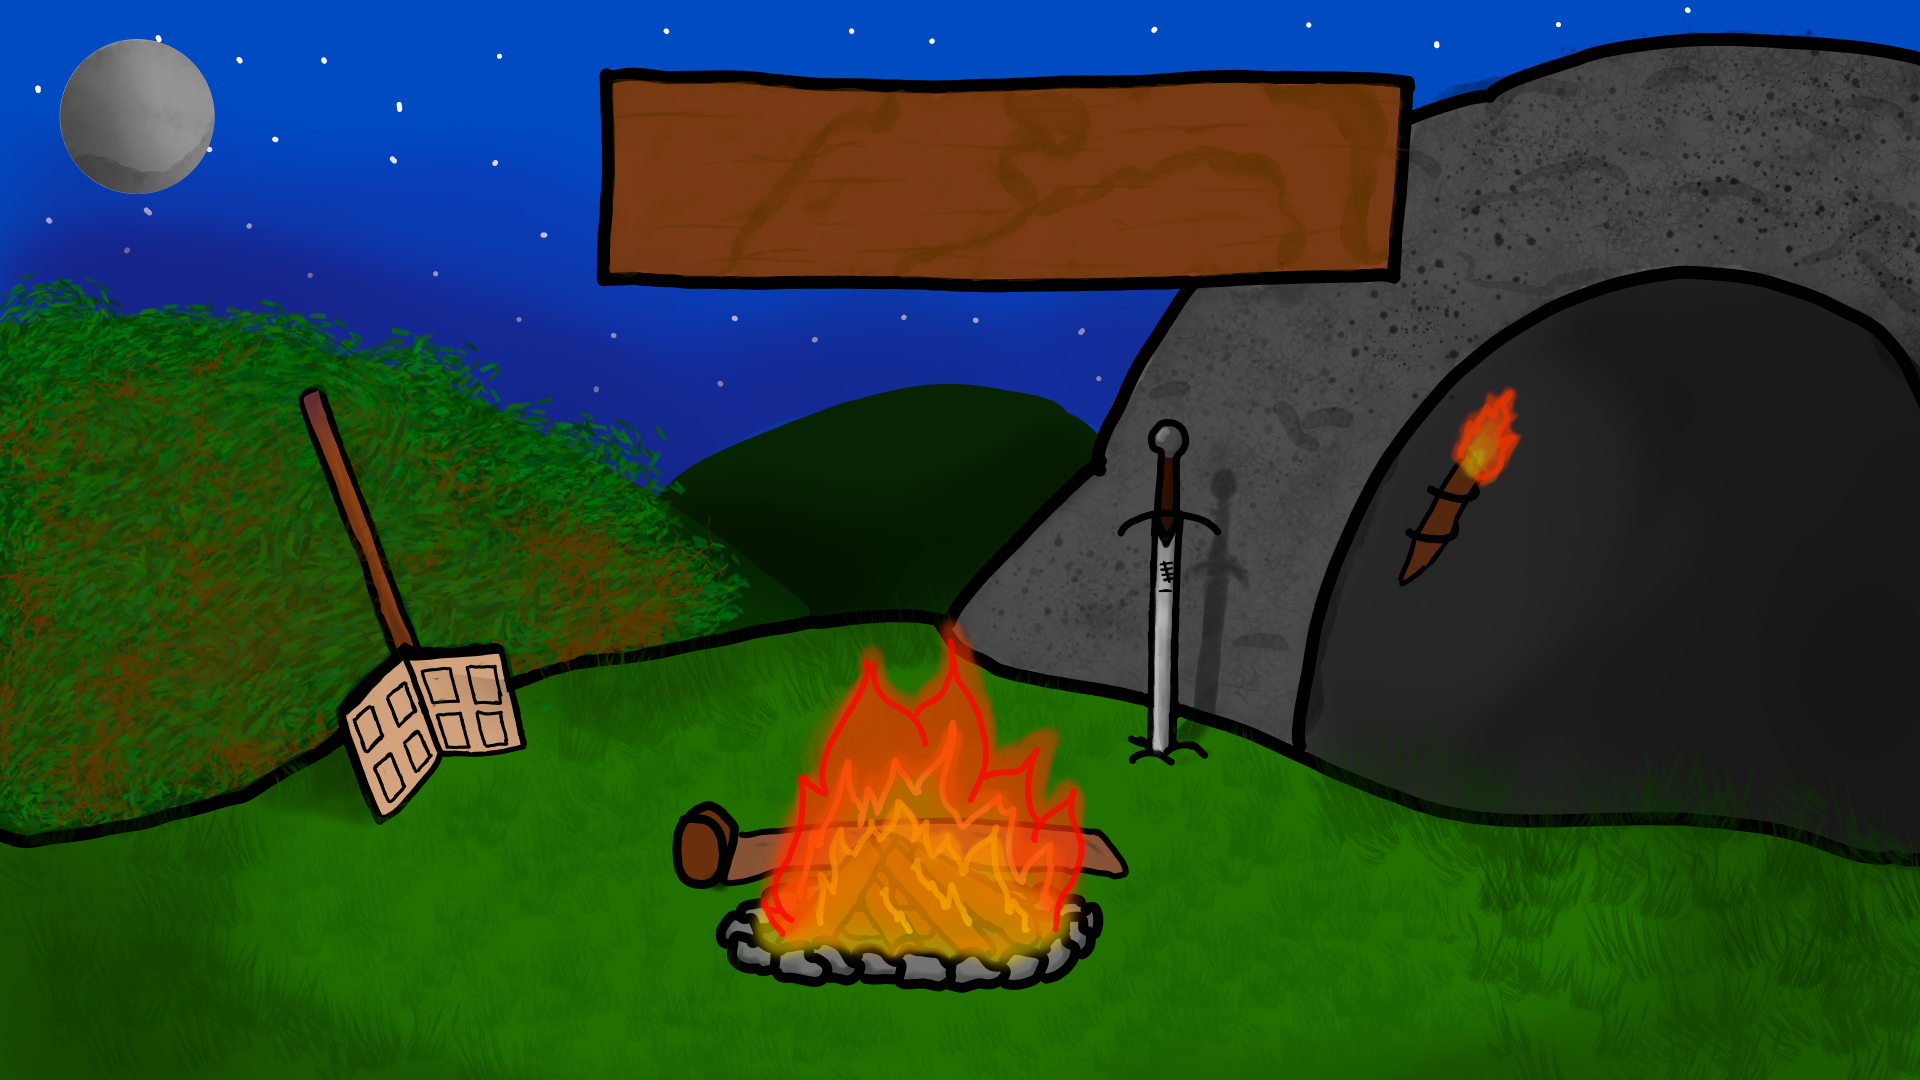
\includegraphics[width=400px,keepaspectratio]{images/Menu.png}
        \caption {A játék menüje}
        \label{Menü}
    \hspace{1em}
\end{figure}
\begin{figure}[h]
        \centering
        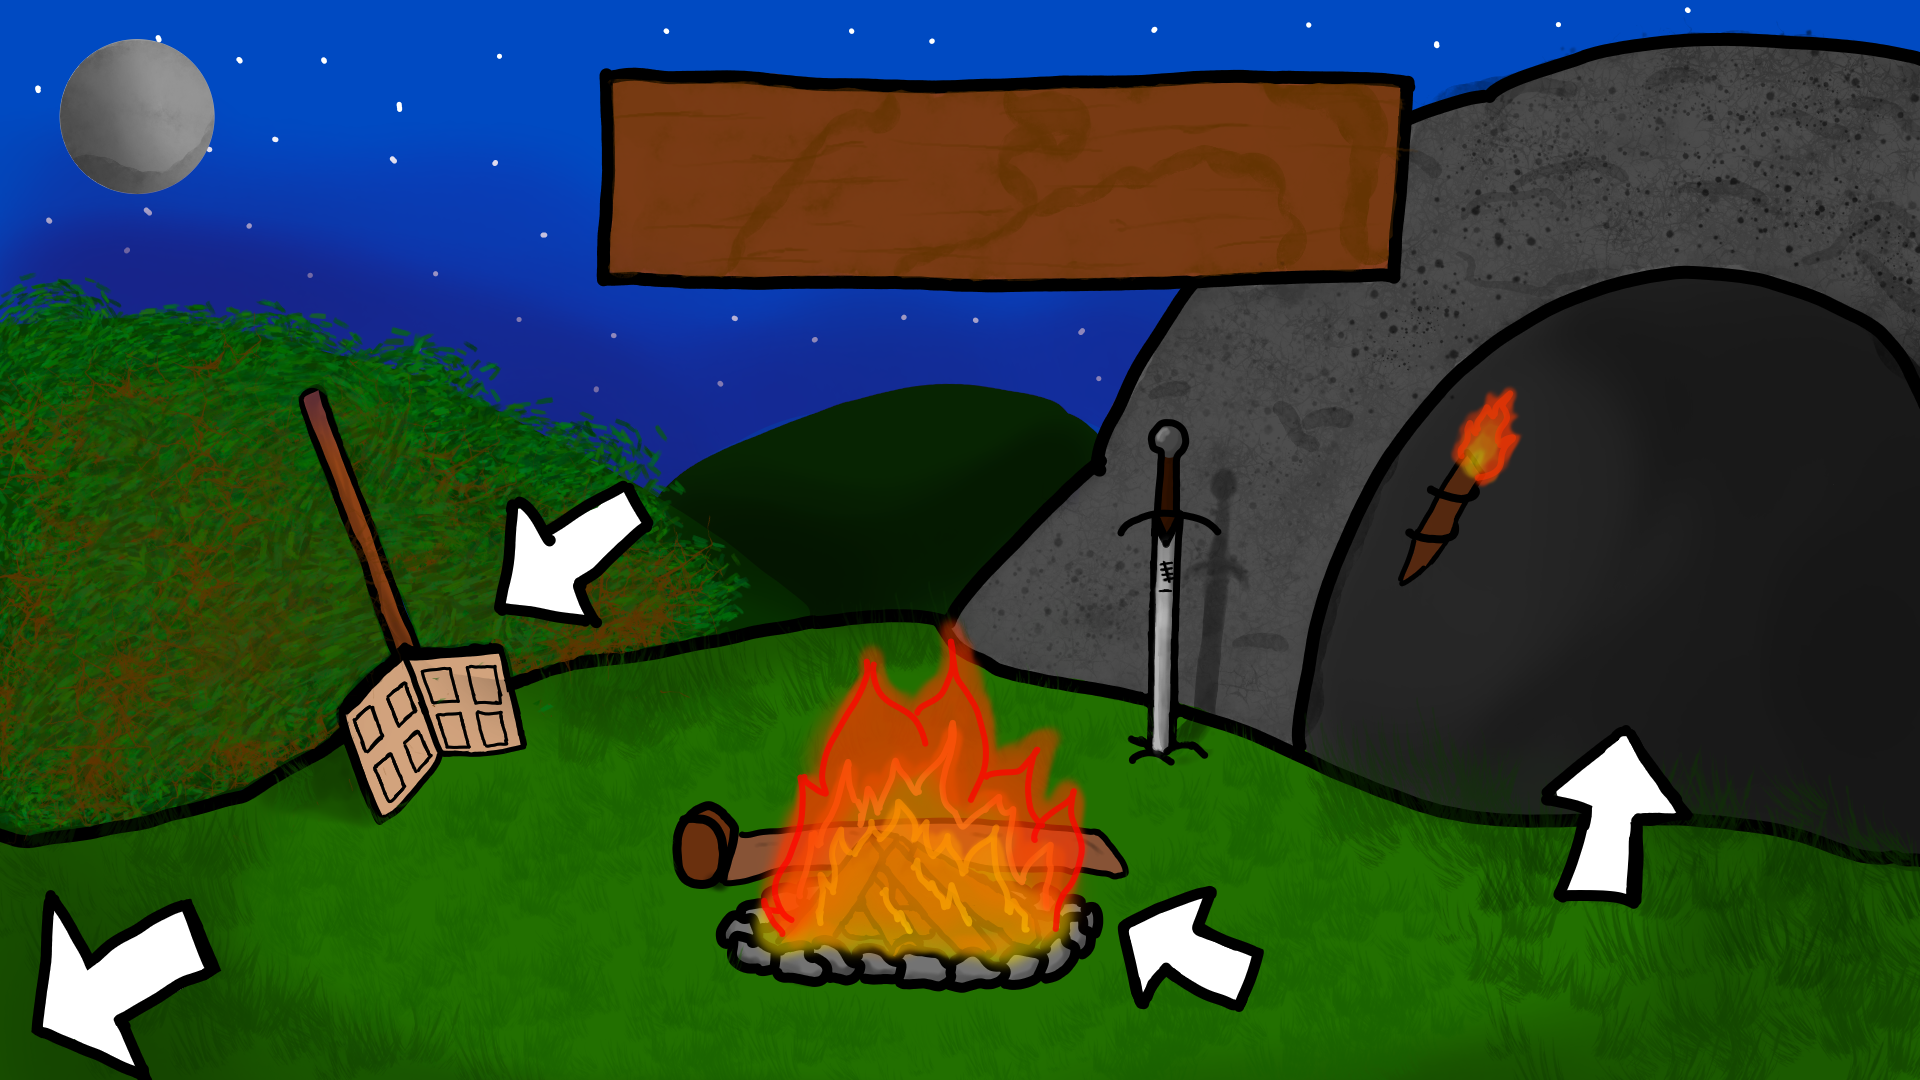
\includegraphics[width=400px,keepaspectratio]{images/menü_with_arrows.png}
        \caption {Interaktív elemek}
        \label{Menü_with_arrows}
    \hspace{1em}
\end{figure}
\clearpage
\subsection{Funkciók}
\subsubsection{Barlang}
A barlangva kattintva idítható el a játék. A játék megkezdése előtt a játékosnak egy Klass-t kell választania. A Klassz választás egy felugró felületen történik ahol mind a 8 Klass meg van jelenítve. A jobb felső sarokban található egy Close gomb amivel be lehet zárni a menüt.
\subsubsection{Tábor tűz}
A tábor tűzre kattintva a játékos a beállítások menübe kerül. Itt tudja a játékos a felbontást beállítani.
\subsubsection{Gyűjtő könyv}
A könyvre kattintva a játékos megnézheti a játékban szereplő kártyákat. Ha a kurzort a kártya felé viszi, a képernyő közepén a kártya megjelenik. A felület két oldalán található egy egy gomb ami lapozási lehetőséget ad a kártyák között. A jobb felső sarokban található a Close gomb amire kattintva a felület bezárja magát.
\subsubsection{Bal Sarok}
A bal sarokba kattintva a játékos kilép a játékból. Ezen felül az Esc gombot lenyomva kiléphetünk az aplikációbol.

\section{Karakter választó}

Miután a főmenüben elindítottuk az új játékot először választanunk kell a játékban
szereplő 8 klass kötül. Ezek mind más-más játékstílussal bírnak a játékos számára.
Miután kiválasztotta a kasztját egy kezdő paklit kap a játékos.
\begin{figure}[h]
        \centering
        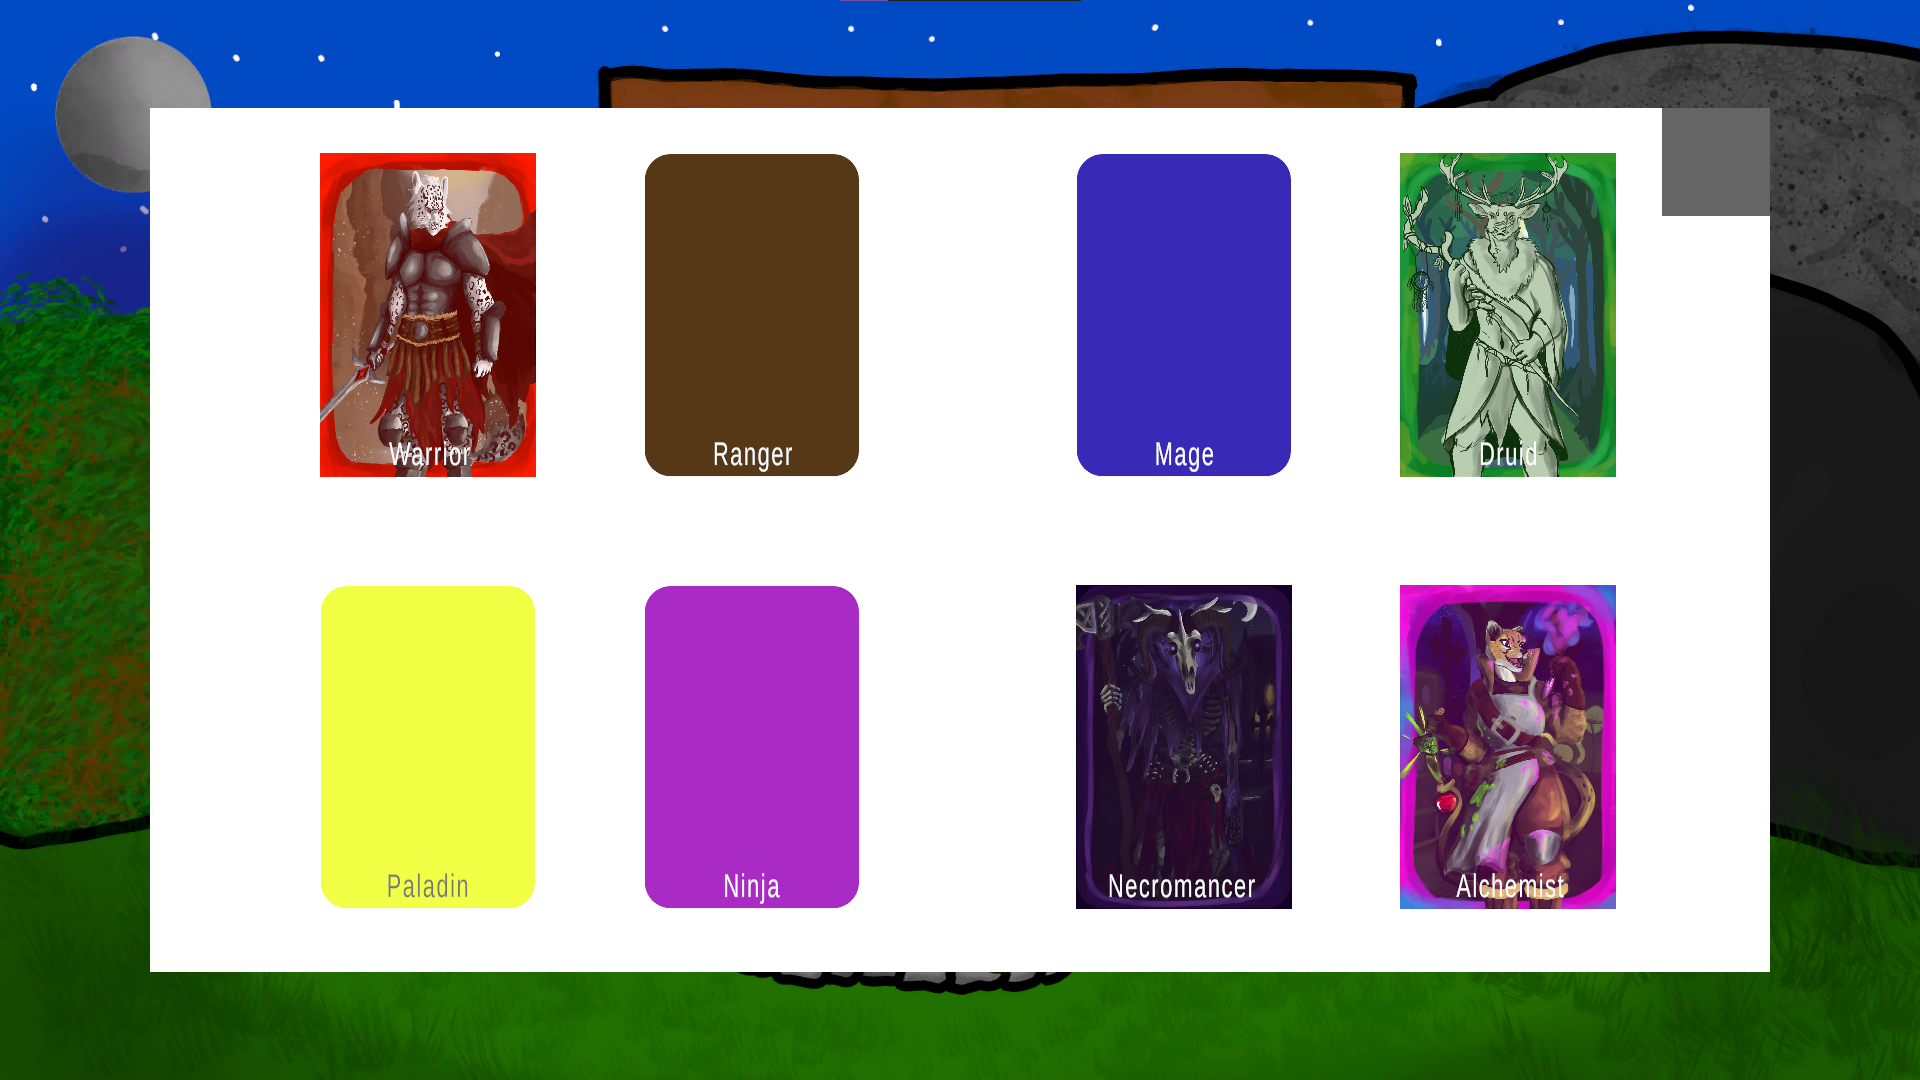
\includegraphics[width=400px,keepaspectratio]{images/CharSelect.png}
        \caption {Karakter választó}
        \label{Karakter_selektor}
    \hspace{1em}
\end{figure}
\clearpage

\section{Aréna}
Miután kiválasztottuk a karakterünket bekerülünk az arénába. Ezen a ponton kezdődik a tényleges játék része az programnak.
\begin{figure}[h]
        \centering
        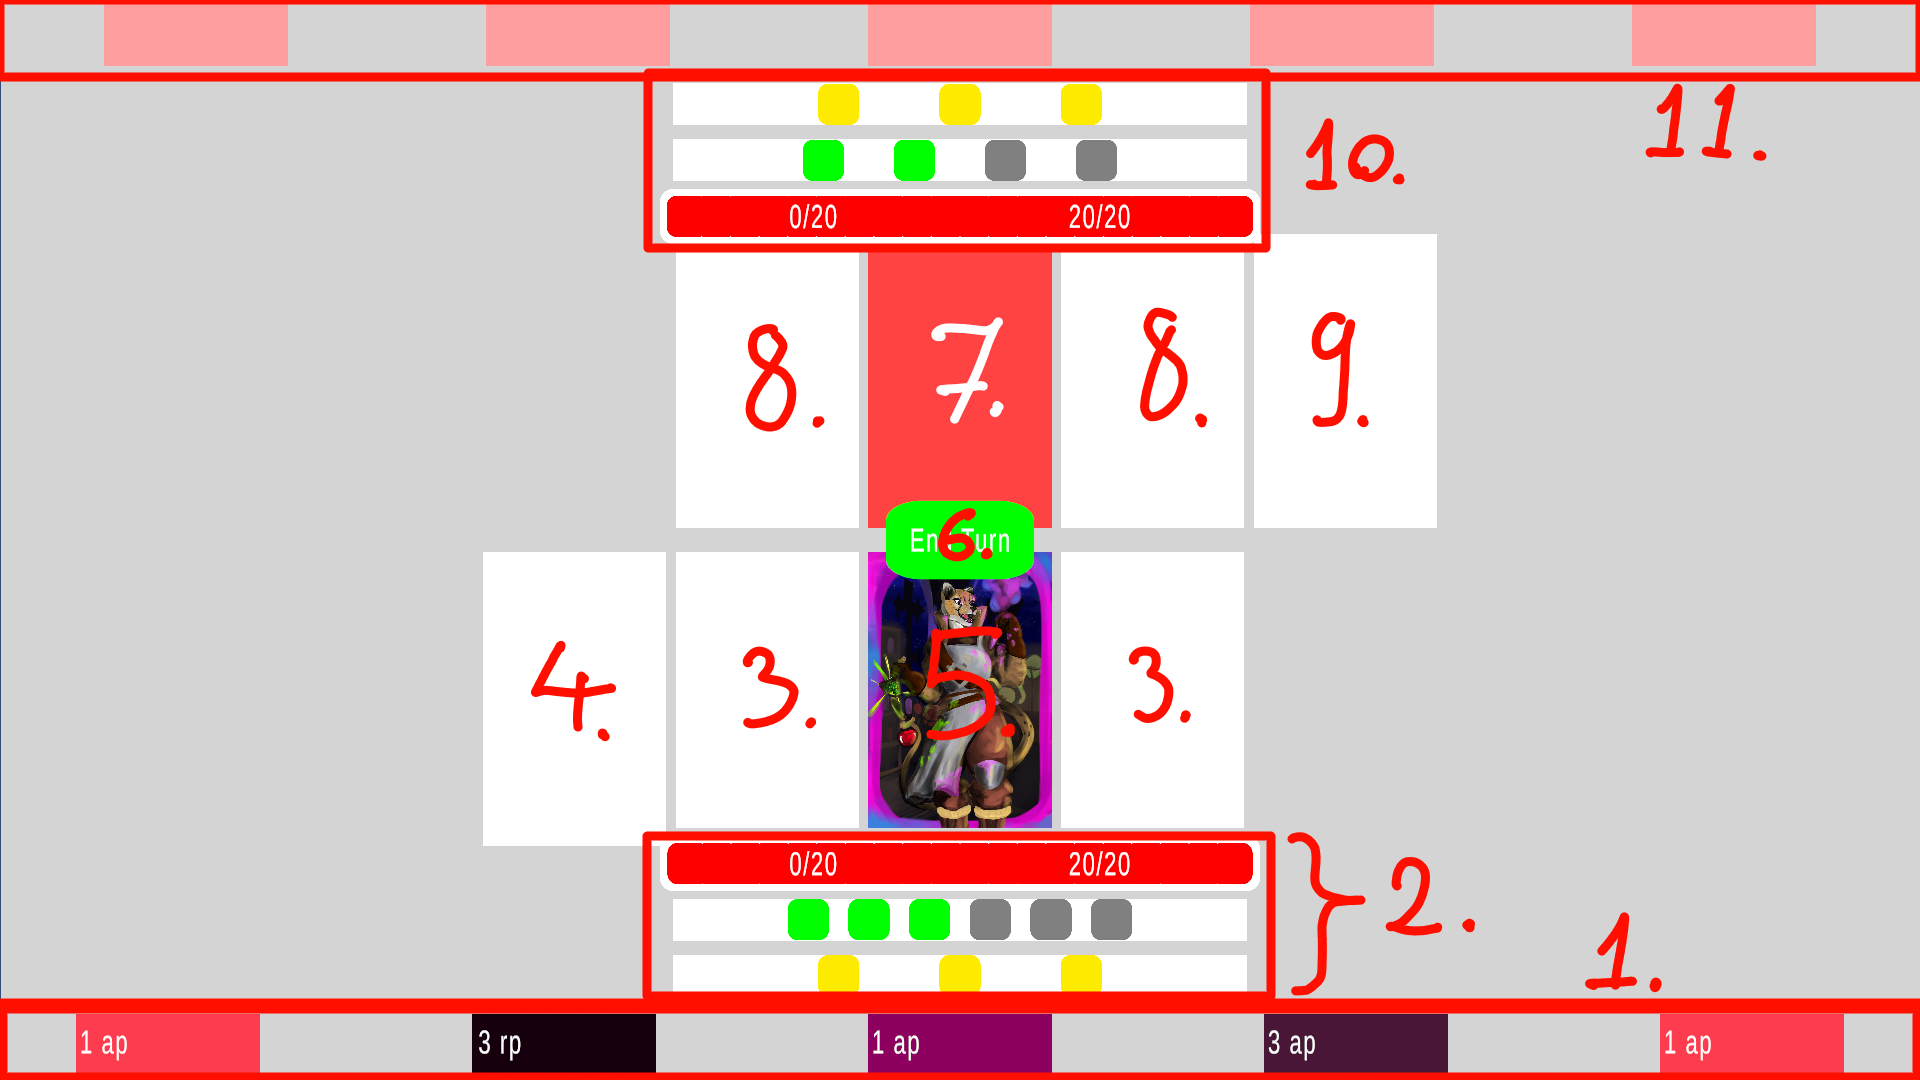
\includegraphics[width=400px,keepaspectratio]{images/BoardExpl.png}
        \caption {Az aréna}
        \label{Arena_full}
    \hspace{1em}
\end{figure}
\subsection{Játékos keze}
Ez a játékos keze. Ide kerülnek a kijátszható lapok a pakliból.
\subsection{Játékos pontjai}
A játékos 4 pontal rendelkezik. Fentről lefelé indulva ezek a:
\begin{itemize}
    \item Pajzs pontok. Ezek mutatják hogy a játékosnak mennyi pajzsa van. A pajzsok csökkentik a beérkező sebzést amit a játékos kapna. Ez a baloldali érték.
    \item Élet pontok. Ezek mutatják meg hogy a játékosnak mennyi maximum életereje illetve jelenleg mennyi életereje van még. Ha ez leesik nullára a játékos veszít. Ez a jobboldali érték.
    \item Akció pontok. Ez az erőforrás egyes kártyák kijátszására használható. Ezek egy részét a játékos visszanyeri a köre elején.
    \item Reakció pontok. Ez az erőforrás más kártyák kijátszására használható fel. a köre elején a játékos visszanyeri az összes reakció pontját.
\end{itemize}
\subsection{Felszerelés és idézett lények}
Ezekbe a kártya helyekbe Felszerelések és idézett lények tehetőek amik segítséget nyújtanak csata közben. Ezek a segítségek lehetnek: a fizikai sebzés növelése, mágikus sebzés növelése, extra sebzés az ellenfélbe, gyógyítás vagy akár extra kártya húzas. 
\subsection{Aréna effectus}
Az aréna effectusok hasnolóak a felszerelésekhez, de csak erre az egy helyre kerülhet. Az aréna effektusok speciális tulajdonságokkal rendelkeznek mint például: a játékos akciópont visszanyerésének növelése vagy pajzs adása akkor hogyha a játékos annyi sebzést szenved el hogy az túlütné a pajzsainak számát.
\subsection{Játékos karaktere}
Itt található a játékos karaktere
\subsection{Kör vége gomb}
Erre rányomva a játékos lezárhatja a körét. Ha zöld a játékos köre van éppen, ha piros akkor pedig az ellenfélé.
\subsection{Ellenfél karaktere}
Ez az ellenfélé karakterének helye.
\subsection{Ellenfél felszerelés}
Ez az ellenfélé felszerelésének helye helye.
\subsection{Ellenfél Aréna effektus}
Ez az ellenfélé aréna effektusának helye helye.
\subsection{Ellenfél pontjai}
Hasonlóan a játékoshoz az ellenfél is rendelkezik: pajzs-, élet-, akció- és reakció pontokkal melyek ugyan úgy működnek mint a játékos pontjai.
\subsection{Ellenfél Kártyáji}
Ez is hasonló a játékos kezéhez az ellenfél a köre során kijátszik kártyákat.
\clearpage

Attól függően hogy az Arénát győztesként vagy vesztesként fejeztük be úgy változik a tovább haladásunk. Ha győztünk egy felugró ablak jelzi számunkra ezt a tényt és a rajta szereplő Continue (folytatás) gombra kattintva tövább léphetünk.

\begin{figure}[h]
        \centering
        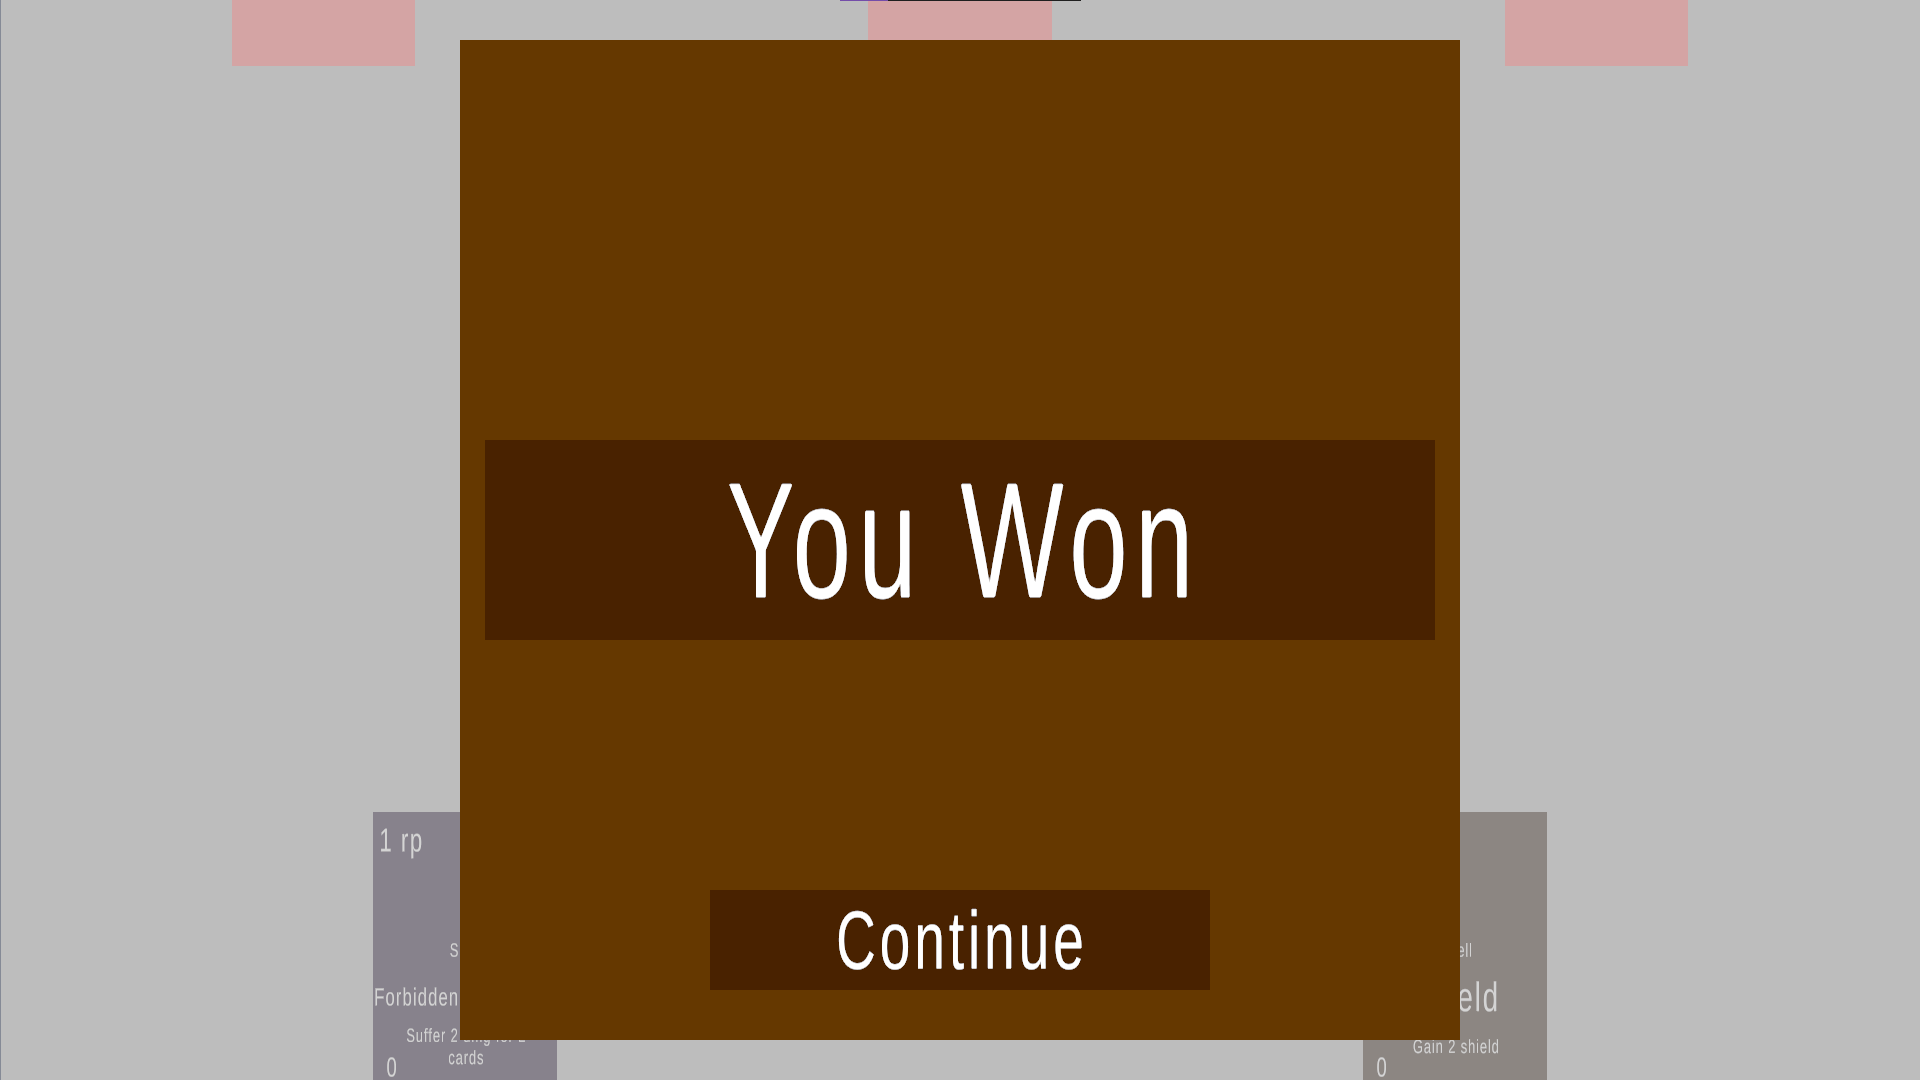
\includegraphics[width=400px,keepaspectratio]{images/won.png}
        \caption {Felugró kép győzelem esetén}
        \label{Won}
    \hspace{1em}
\end{figure}

Ha vesztettünk akkor egy hasonló ablak vár minket ami közli velünk hogy vesztettünk és egy gomb ami pedig vissza visz minket a főmenübe ahol újra kezdhetjük a kalandunkat. 

\begin{figure}[h]
        \centering
        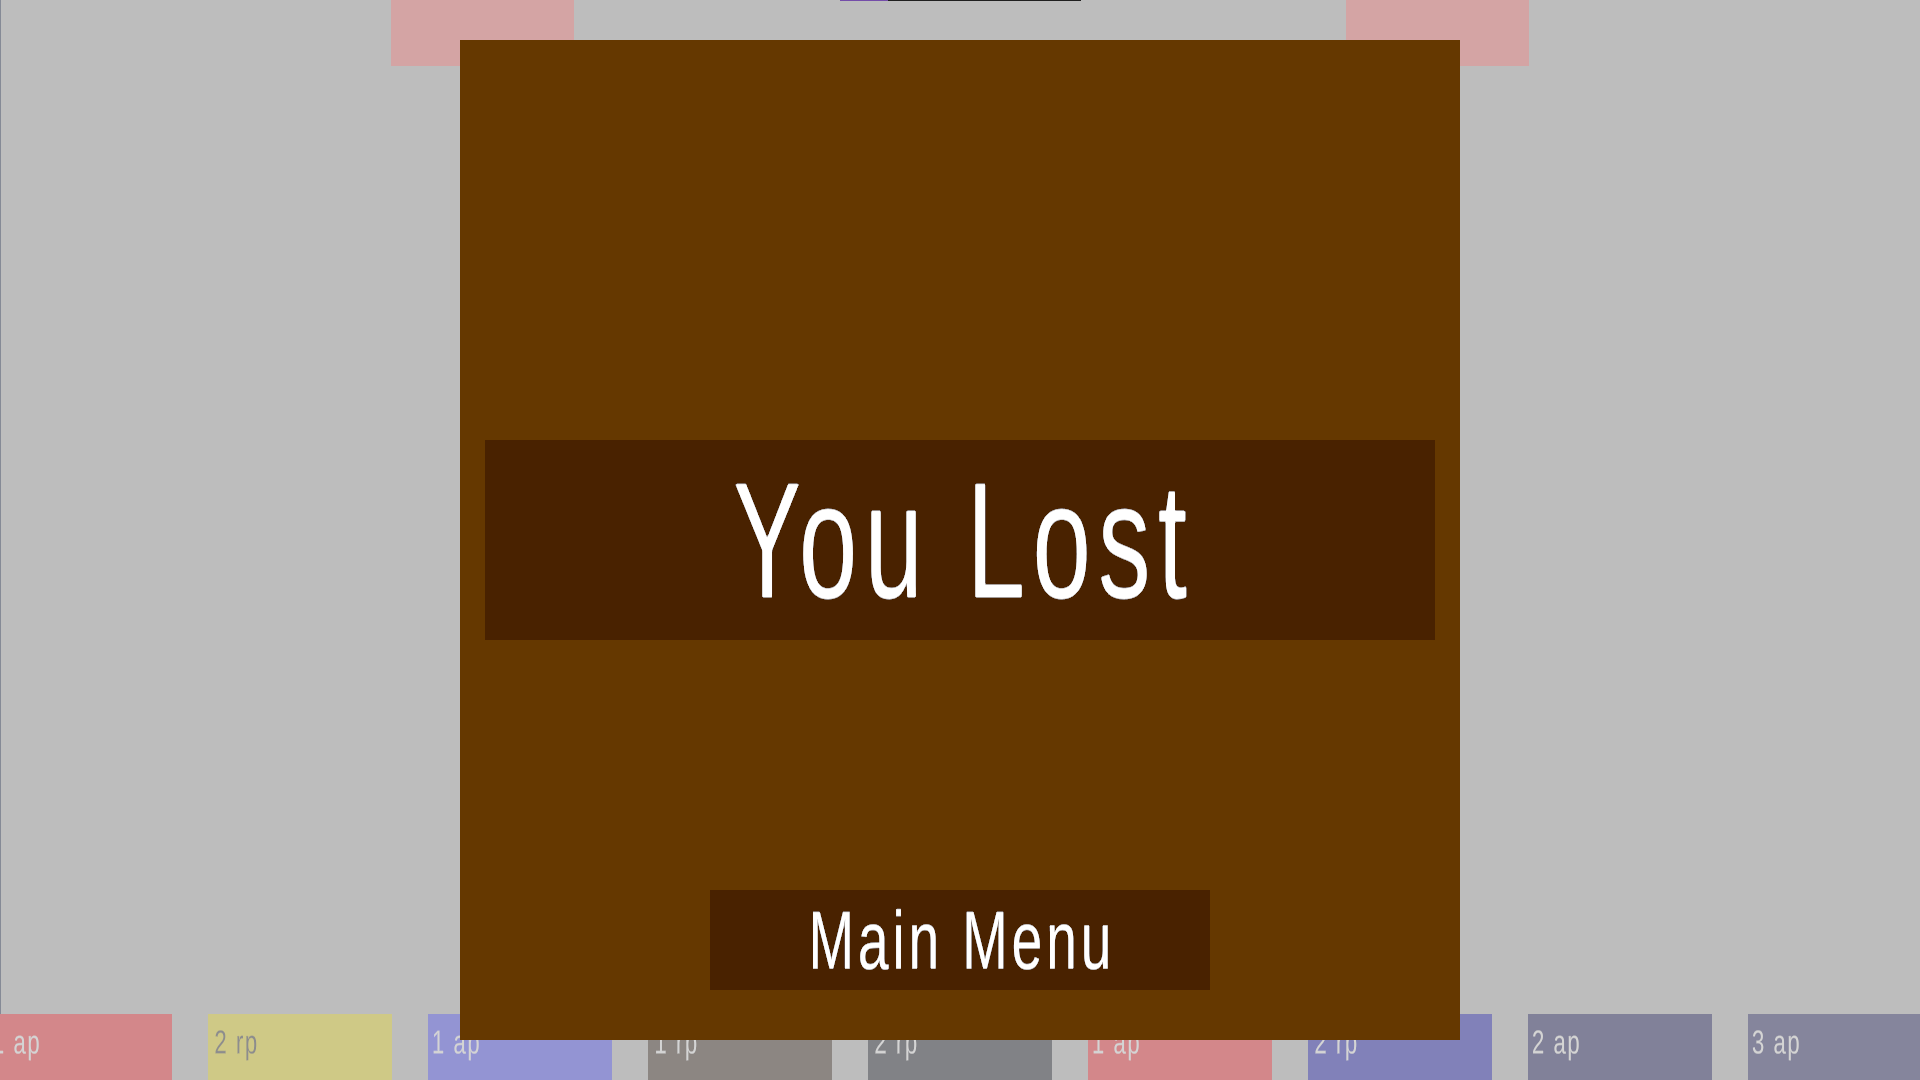
\includegraphics[width=400px,keepaspectratio]{images/lost.png}
        \caption {Felugró kép vesztés esetén}
        \label{lost}
    \hspace{1em}
\end{figure}

\clearpage
\section{Kártya Választás}

Miután nyertünk tovább kerülünk a kártya választó felületre. Itt bővíthatjük a meglévő paklinkat és ezzel a randelkezésünkre álló kombókat. Egyszerre mindíg 4 kártyát látünk a képernyőn, ezeket a jobb és bal oldalon elhelyezkedő nyilakkal tudjuk változtatni. Kattintással ki tudjuk választani a kártyát amit szeretnénk hozzáadni a paklinkhoz. Ha kiválasztottunk egy kártyát akkor egy sárgás színt vesz fel ezzel jelezve hogy ki van választva. A Finalize gombra kattintva tovább léphetünk a következő csatára.

\begin{figure}[h]
        \centering
        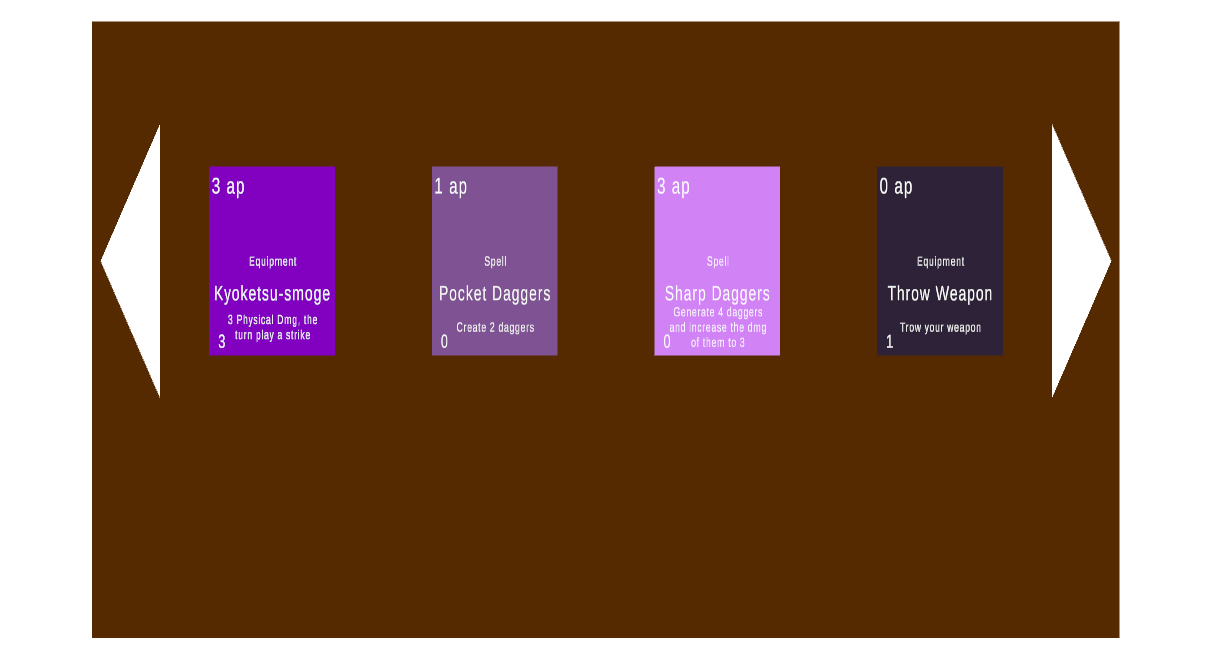
\includegraphics[width=400px,keepaspectratio]{images/chooseCard.png}
        \caption {A menü ahonnan a kártyát választjuk}
        \label{Choose}
    \hspace{1em}
\end{figure}

\begin{figure}[h]
        \centering
        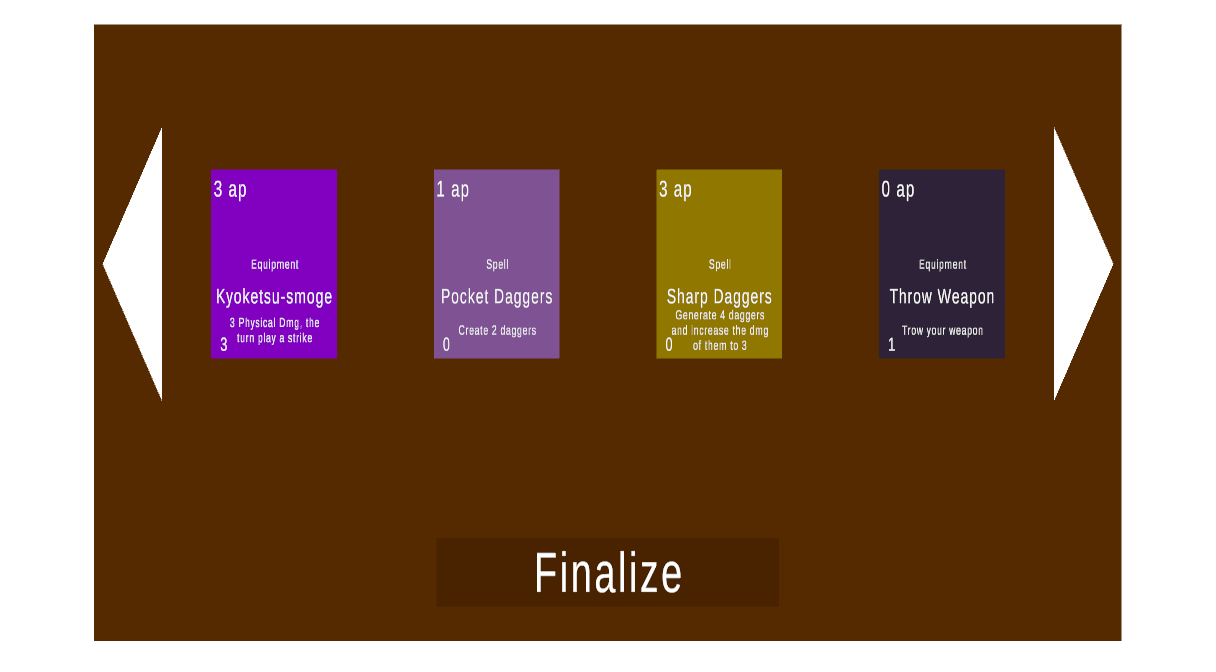
\includegraphics[width=400px,keepaspectratio]{images/cardChoosen.png}
        \caption {A menü kártya választás után}
        \label{Chosen}
    \hspace{1em}
\end{figure}

\chapter{Játékmenet}

\section{Játék elkezdése}
A játék elkezdéséhez rá kell kattintanunk a barlangra. Miután rákattintottunk a barlangra az új játék megkezdéséhez választanunk kell egy karakter klasst. Ezek mind más-más játékstílussal bírnak a játékos számára. Miután kiválasztottuk a karaktert kapunk egy kezdő paklit. Ez a pakli 5 darab egyedi kártyából melyek a klass saját kártyái illetve 4 mindenki számárá elérhető kártyából áll. Ez a 4 kártya 2 Strike, 1 Draw és 1 Defend kártyából áll.

\subsection{Kasztok}
\begin{itemize}
        \item Warrior avagy a Harcos:\\\
        Agresszív támadás orientált játékstílus. Fő fókuszban a Strike kártyák álnak és ezeknek az erősítése. A klass 2 felszereléssel, és 3 varázslak kártyával rendlekezik. 
        \item Ranger avagy az Íjjász: \\\
        Hibrid kombinációja az agresszív támadás orientált és passzívabb önerősítő játékstílusnak. A Ranger kombinálja a felszereléseinek támadási előnyeit az aréna effektusok kontrolláló képességeivel. A klass 2 felszereléssel, 1 varázslattal és 2 aréna effektussal operál. 
        \item Mage  avagy a Mágus: \\\
        Varázslat orientált passzívabb játékstílus. Ereje a varázslatok erősítésében és a támadások mágiával való kombinációjában rejlik. A klass 2 varázslattal, 2 felszereléssel és 1 aréna effektussal rendelkezik.
        \item Paladin avagy a Lovag: \\\
        Passzív védelem és pajzs orientált játékstílus. A Paladin képes a pajzsát sebzésre használni.  A klass 3 varázslattal, 1 felszereléssel és 1 aréna effektussal rendelkezik.
        \item Druid avagy a Druida:\\\
        Passzív öngyógyítás és gyógyulás közbeni mágikus sebzésre épülő játékstílus. A Druid fő erőssége hogy konzisztensen tudja magát gyógyítani és támadni is egyszerre. A klass 2 varázslattal, 1 felszereléssel és 2 aréna effektussal rendelkezik.
        \clearpage
        \item Ninja  avagy a Nindzsa:\\\
        Agresszív támadás és Token generálásra épülő játékstílus. A ninja erejét a dobókései adják melyeket képes generálni illetve erősíteni kártyáiva. A klass 3 varázslattal és 2 felszereléssel rendelkezik.
        \item Necromancer avagy a Nekromanta:\\\
        Agresszív játékstílus a idézett csontváz katonákra és élet pont felhasználásra építve.
        A Nekromancer az idézett élőhalott katonájival képes nagy fizikai és mágikus sebzést kiosztani illetve életpontjait felhasználni kártyák szerzésére. A klass 2 varázslattal és 2 idézett lénnyel és 1 aréne effektussal rendelkezik.
        \item Alchemist avagy az Alkemista\\\
        Agresszív kártya generálásra épülő játékstílus. Az Alchemist fő erőssége a főzetei amikor sokrétű képességekkel rendelkeznek. A klass 3 varázslattal és 2 felszereléssel rendelkezik.
\end{itemize}

\section{Játék az arénán belül}

Amint kiválasztottuk a klasst amivel játszani szeretnénk bekerülünk az arénába. A játék körökre van osztva. A játékos kezd. Az első körben a játékos felhúz 5 lapot, 4 kezdő lapot és plusz 1 lapot amit minden kör elején felhúz. Ezeket a lapokat a játékos a köre során tudja kijátszani. A kártyák sokmindenre képesek. Vannak amelyek csak egyszerű támadás kártyák amik az ellenfelet sebzik míg mások egyszer felhasználható úgynevezett Token kártyákat hoznak létre 

Ha a játékos befejezte a kötét akkor a középen található End turn gombra kattinva lezárhatja a körét. Amint a játékos lezárta a körát az esetleges kör végi effektusok érvényesülnek majd az ellenfél köre következik. Az ellenfél a köre elején felhúzza lapjait majd kijátsza őket. Miután végzett a körével újra a játékos köre következik. Ekkor a játékos visszanyeri az akció pontjainak egy részét, a reakciópontjait illetve az esetleges kör eleji effektusok életbe lépnek. Fontos megemlíteni hogy a játékos kezében nem lehet több mint 10 kártya egyszerre.

Ez mind addig megy így ameddig a játékos le nem viszi az ellenfele életét nullára vagy pedig a játékos saját életpontjainak száma el nem éri a nullát. Ha a játékosnak sikerül az ellenfele életpontjait leredukálni nullára akkor a játékos megnyerte a csatát és tovább léphet. Ha a játékos sikertelen volt és az ellenfél leredukálta a játékos életpontjainak számát nullára akkor a játékos vesztett.

\subsection{Győzelem}
Ha a játékos győzött akkor tovább kerül a kártya választó képernyőre ahol kibővíthati a pakliját egy tetszőleges kártyával. Miután a játékos rákattintott a kivánatos kártyára a Finalize gomb megjelenik és arra kattintava a játékos visszakerül az arénába ahol folytathatja a harcolást.

\subsection{Veszítés}
Ha a játékos veszített akkor egy felugró ablak értesíti hogy vesztett és a Main Menu gombra kattintva vissza kerül a Fő menübe.

\begin{figure}[h]
        \centering
        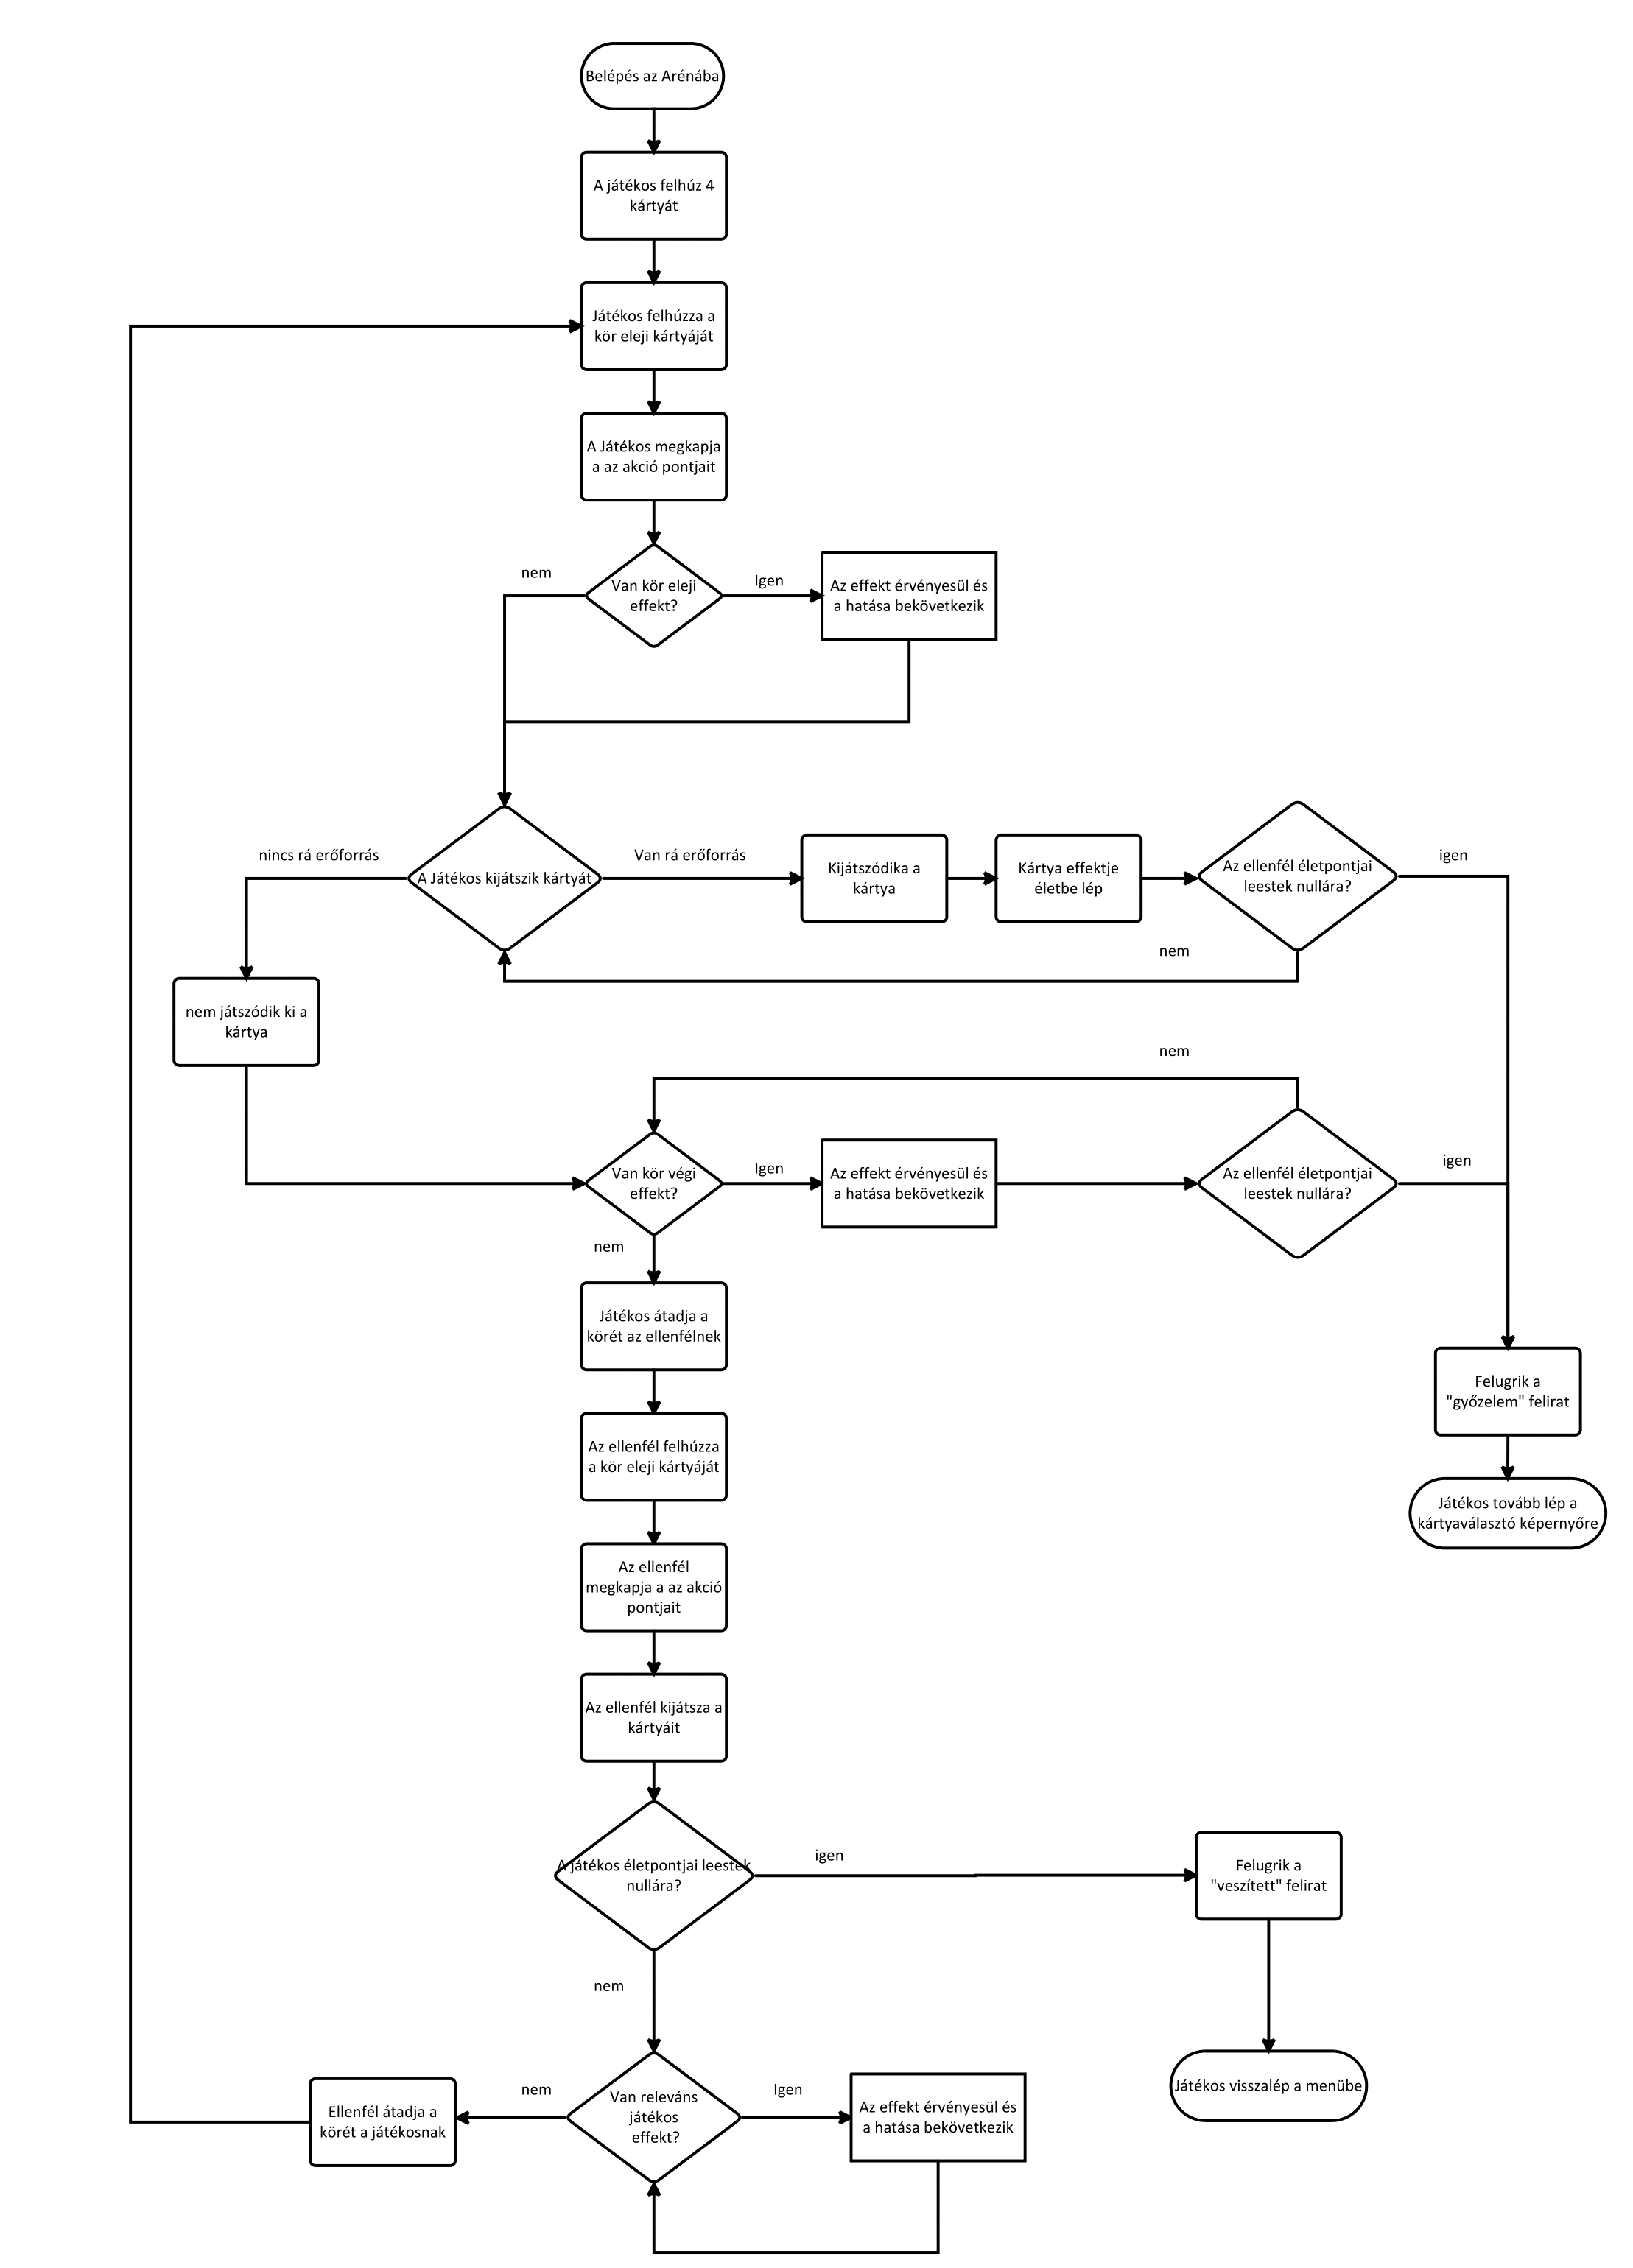
\includegraphics[width=420px,keepaspectratio]{images/Gameplay.png}
        \label{GamplayChart}
        \caption {A játékmenet folyamat ábrája}
    \hspace{1em}
\end{figure}

\chapter{A kártyák}

A játék egyik ha nem legfontosabb eleme a kártyák. Összesen a játék 44 egyedi kártyát tartalmaz. Karakter klassonként 5 kártyát és 4 klass függetlent. Fontos a kártyák színe ami a klasshoz való tartozásukat szimbolizálja. Ezek a színek a :\\\
     Warrior - Piros és árnyalatai \\\
     Ranger - Barna és árnyalatai\\\
     Mage - Kék és árnyalatai\\\
     Paladin - Sárga és árnyalatai\\\
     Druid - Zöld és árnyalatai\\\
     Ninja - Lila és árnyalatai\\\
     Necromancer - Sötét Lila és Szürkék\\\
     Alchemist - Rózsaszín és árnyalatai\\\

\section{Kártya Típusok}
A játék 5 nagy kártya típussal operál: Felszerelés, Varázslat, Aréna Effektus, Idézett lény és Token. Ezek más más tulajdonságokkal bírnak és máshogy működnek.
\begin{itemize}
    \item Felszerelés:\\
    Álatlánosan a játékosnak ad fizikai vagy mágikus bónusz sebzést. Ezek a játékos karakterétől jobbra és barra lévő helyekre lehet lehelyezni.
    \item Varázslat:\\\
    Ezek a kártyák kijátszáskor valamit csinálnak. Ez lehet sebzés, gyógyítás, kártyahúzás stb.
    \item Aréna Effektus:\\\
    Passzív effektekkel bírnak melyek vagy a kör elején vagy a végén akitválódnak.
    \item Idézett lények:\\\
    Ezek a Felszereléshez hasonlőan működnek de a sebzés bónuszon túl azzal a tulajdonsággal bírnak hogy együtt támadnak a játékossal.
    \item Token:\\\
    A Tokenek a Varázslatokhoz hasonlóak annyi külömbséggel hogy egyszehasználatosak, kártyák generálják őket, a sebzésük nem függ a játékos fizikai és vagy mágikus sebzés bónuszától illetve nem kerülnek semmilyen pontba. 
\end{itemize}

\section{Kártya felépítése}
\subsection{Proof of concept}
\begin{itemize}
    \item A bal felső sarokban látható a kártya ára. A zöld gömb az akció pontot jelenti, a sárga háromszög pedig a reakciópontot. A mennyiség pedig hogy mennyi pontba kerül a kártya.
    \item Középen található a kártya neve.
    \item A név felett található egy kis rajz a kártyához illetve a keret. A keret határozza meg illetve közli a játékossal hogy milyen típusú kártyáról van szó. Hatszög szerű = felszerelés, ovális = aréna effektus, stb.
    \item A név alatt található a kártya leírás.
    \item A bal alsó sarokban található a sebzés értéke a kártyának.
\end{itemize}

\subsection{Place Holder}
\begin{itemize}
    \item A bal felső sarokban látható a kártya ára. Először a mennyiség szerepel majd a pont típusa
    \item Középen található a kártya neve.
    \item A név felett található a kártya típusa. Ezek lehetnek: Varázslat, Felszerelés, Aréna Effeckt, Idézett lény, Token.
    \item A név alatt található a kártya leírás.
    \item A bal alsó sarokban található a sebzés értéke a kártyának.
\end{itemize}

A kártyák a jövőben hasonlóan néznének ki a Sword számára elkészült rajz.

\begin{figure}[h]
        \centering
        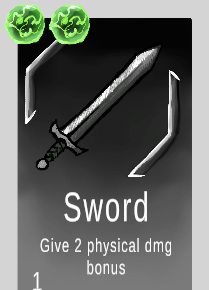
\includegraphics[width=140px,keepaspectratio]{images/SwordPic.png}
        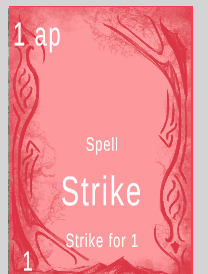
\includegraphics[width=140px,keepaspectratio]{images/Strike.png}
        \label{POC}
        \caption { Koncepció a tényleges kártyákról és a place holder kártya}
    \hspace{1em}
\end{figure}

\section{Általános}

\begin{itemize}
    \item Strike - Varázslat\\\
    - Ára: 1 akció pont \\\
    A kártya 1 + fizikai sebzés bónusz sebzést okoz az ellenfélnek.
    \item Defend - Varázslat\\\
    - Ára: 1 reakció pont \\\
    A játékos 2 pajzspontot kap.
    \item Draw - Varázslat\\\
    - Ára: 2 reakció pont \\\
    A játékos húz egy kártyát.
    \item Sword - Felszerelés\\\
    - Ára: 2 akció pont \\\
    Egy szimpla kard  ami 2 bónusz fizikai sebzést ad.
\end{itemize}

\section{Warrior}
\begin{itemize}
    \item Blood Thirster - Felszerelés:\\\
    - Ára: 2 akció pont \\\
    A kártya plusz 1 fizikai sebzés bónuszt kap az összes ebben a körben az összes kijátszás előtt kijátszott Strike ért. Ebbe bele tartozik a Fury Strike (plus annyi Strike ahányszor a kártya aktiválódott), Double Strike (plus 2) és a Throw Weapon is. 
    \item Flesh Ripper - Felszerelés:\\\
    - Ára: 3 akció pont \\\
    Ha a játékos Strike-ot játszik ki akkor a támadás előtt elpusztítja az ellenfél 2 pajzspontját majd utána támad.
    \item Double Strike - Varázslat\\\
    - Ára: 2 akció pont \\\
    A játékos kétszer kijátsza a Strike-ot.
    \item Fury Strikes - Varázslat\\\
    - Ára: x akció pont \\\
    A játékos annyi Strike kártyát játszik ki ammenyi elérhető akció pontja van. Mindegy egyes kijátszott Strike után elkült 1 akció pontot.
    \item Battle Rage - Varázslat\\\
    - Ára: 1 reakció pont \\\
    A játékos ebben a körben kap 2 bónusz fizikia és mágikus sebzést.
\end{itemize}

\clearpage
\section{Ranger}
\begin{itemize}
    \item Ranger Bow - Felszerelés:\\\
    - Ára: 1 akció pont \\\
    A kártya plus 1 fizikai sebzés bónuszt ad.
    \item Crossbow - Felszerelés:\\\
    - Ára: 3 akció pont \\\
    A kártya plus 3 fizikai sebzés bónuszt ad illetve minden kör elején ad egy extra akció pontot..
    \item Aroow Volley - Varázslat:\\\
    - Ára: 2 akció pont \\\
    A kártya kilő 4 + a fizikai és mágikus bónusz sebzés darab nyilat melyek mind 1 sebzést okoznak. 
    \item Wind Sweapt Hills - Aréna Effektus:\\\
    - Ára: 2 reakció pont \\\
    Ha a kártya aktív a játékos a köre elején egy extra lapot húz fel.
    \item Hunters Trap - Aréna Effektus:\\\
    - Ára: 2 akció pont \\\
    Ha az ellenfél megtámadja a játékost akkor az ellenfél elszenved 1 sebzést.
\end{itemize}

\section{Mage}
\begin{itemize}
    \item Sorcefull Staff - Felszerelés:\\\
    - Ára: 2 akció pont \\\
    A kártya plus 3 mágikus sebzés bónuszt ad. Ha a felszerelés használva van akkor a Strike kártyák sebzéséhez hozzá adódik a játékos mágikus sebzés bónusza is. 
    \item Arcane Spellbook - Felszerelés:\\\
    - Ára: 2 reakció pont \\\
    A kártya plus 1 mágikus sebzés bónuszt ad. Amíg a kártya a táblán van a játékos minden egyes kijátszott vatázslat után felhúz egy kártyát.
    \item Arcane Spike - Varázslat:\\\
    - Ára: 1 akció pont \\\
    A kártya kioszt 1 sebzést 3 + bónusz mágikus sebzés szer.
    \item Magic Missle - Varázslat:\\\
    - Ára: 3 akció pont \\\
    A játékos előkészít egy hatalmas mágikus csapást. Ez a támadás a játékos bónusz mágikus sebzésének három szorosát sebzi az ellenfélbe.
    \item The Storm - Aréna Effektus:\\\
    - Ára: 2 reakció pont \\\
    Ha ez a kártya a pályán van akkor a játékos általi támadások (akár levédi az ellenfél pajzsa akár nem) 1 sebzést okoznak azonnal az ellenfél életpontjainak.
\end{itemize}

\section{Paladin}
\begin{itemize}
    \item Paladin Shield - Felszerelés:\\\
    - Ára: 2 reakció pont \\\
    A kör elején a játékos kap egy pajzs pontot.
    \item Provoke - Varázslat:\\\
    - Ára: 1 akció pont \\\
    Kijátszáskor a játékos egy pajzs pontot kap illetve húz egy kártyát.
    \item Holy Block - Varázslat:\\\
    - Ára: 2 reakció pont \\\
    Amikor a játékos kijátsza ezt a kártyát azonnal 5 pajzs pontot kap. Ezen felül 2 mágikus sebzés bónuszt kap erre a körre.
    \item Shield Throw - Varázslat:\\\
    - Ára: 2 akció pont \\\
    A játékos a pájzsát használva az offenzívára tör. Az ellenfél annyit sebződik amennyi pajzsa van a játékosnak.
    \item Mountain Stance - Aréna Effektus:\\\
    - Ára: 3 reakció pont \\\
    Ha a játékos több sebzést ka mint amennyi pajzs pontja van akkor kap 1 pajzs pontot.
\end{itemize}

\section{Druid}
\begin{itemize}
    \item Druid Staff - Felszerelés:\\\
    - Ára: 2 akció pont \\\
    A kártya plus 3 mágikus sebzés bónuszt ad. A kör elején gyógyítja a játékost 1 + mágikus sebzés búnusz mennyiséggel.
    \item Visous Veins - Aréna Effektus:\\\
    - Ára: 2 akció pont \\\
    Agresszív gyökerek körbeveszik az ellenfelet. Az ellenfél a köre elején elveszít egy akció pontot illetve a gyökerek elpusztítjék2 pajzs pontját.
    \item Forest Of Favours - Aréna Effektus:\\\
    - Ára: 3 reakció pont \\\
    Ha a kártya a pályán van a játékos a köre elején gyógyul 1 + mágikus sebzés búnusz mennyiséget és kap egy extra akciópontot.
    \item Woddland Mending - Varázslat:\\\
    - Ára: 2 akció pont \\\
    A játékos gyógyul 3 + mágikus sebzés búnusz mennyiséget míg az ellenfél elszenved ugyan ennyit.
    \item Meditation - Varázslat:\\\
    - Ára: 3 akció pont \\\
    A játékos felhúz egy kártyát. A következő köben felerősíti magát. A Kört 2 extra akció pontal kezdi illetve kap 3 mágikus sebzés bónusz erre a körre. 
\end{itemize}

\section{Ninja}
\begin{itemize}
    \item Kunai - Felszerelés:\\\
    - Ára: 1 akció pont \\\
    A kártya plus 1 fizikai sebzés bónuszt ad. A kör elején generál egy Dagger Token kártyát.
    \item Kyoketsu-smoge - Felszerelés:\\\
    - Ára: 3 akció pont \\\
     A kártya plus 3 fizikai sebzés bónuszt ad. A Kör végén a körben kijátszott 
     Strike-ok + 1-el egyenlő mennyiségű sebzést okoz az ellenfélnek.
    \item Pocket Daggers - Varázslat:\\\
    - Ára: 1 akció pont \\\
    Generál 2 Dagger kártyát a játékos kezébe.
    \item Sharp Daggers - Varázslat:\\\
    - Ára: 3 akció pont \\\
    Generál 4 Dagger Kártyát a játékos kezébe. Ebben a körben a Dagger kártyák sebzése 1-ről 3-ra nő
    \item Weapon Throw - Felszerelés:\\\
    - Ára: 0 akció pont \\\
    A Játékos eldobja az egy felszerelését és ezzel Strike-ol egyet.
    \item Dagger - Token:\\\
    - Ára: 0 akció pont \\\
    A kártya kijátszáskor 1-et sebez az ellenfélbe.
\end{itemize}

\section{Nercomancer}
\begin{itemize}
    \item Bob - Idézett lény:\\\
    - Ára: 3 akció pont \\\
    Bob egy feltámasztott csontváz katona, 3 fizikai sebzés bónuszt ad és ha a játékos Strike kártyát játszik ki akkor megtámadja az ellenfelet és 2 sebzést okoz.
    \item Harly - Idézett lény:\\\
    - Ára: 3 reakció pont \\\
    Harly egy feltámasztott csontváz Mágus, 3 mágikus sebzés bónuszt ad és ha a játékos Strike kártyát játszik ki akkor megtámadja az ellenfelet és 2 sebzést okos.
    \item Decaying Touch - Varázslat:\\\
    - Ára: 2 akció pont \\\
    A játékos 3 + mágikus sebzés bónus sebzést okoz az ellenfelénel és ezt a sebzést vissza gyógyítja magán.
    \item Forbidden Knowledge - Varázslat:\\\
    - Ára: 1 reakció pont \\\
    A játékos feláldoz 2 élet pontot és ezért felhúz 2 lapot.
    \item The Graveyard - Aréna Effektus:\\\
    - Ára: 1 reakció pont \\\
    A játékos a körei végén kap 2 pajzs pontot.
\end{itemize}

\section{Alchemist}
\begin{itemize}
    \item Alchemists gloves - Felszerelés:\\\
    - Ára: 3 reakció pont \\\
    A kör elején kreál egy potiont a játékos kezébe. Az első kijátszott Potion kártyáról csinál egy másolatot a játékos kezébe.
    \item Potion launcher - Felszerelés:\\\
    - Ára: 3 akció pont \\\
     A kártya plus 1 mágikus sebzés bónuszt ad. A játékos köre elején a kártya kijátszik 3 random Potion kártyát.
    \item Home Brewing - Varázslat:\\\
    - Ára: 1 akció pont \\\
    Kreál a játékos kezébe 2 random Potion Kártyát. 
    \item Potion Potion - Varázslat:\\\
    - Ára: 3 akció pont \\\
    Kreál a játékos kezébe egyet az összes Potion kártyából.
    \item Recycling - Varázslat:\\\
    - Ára: 1 reakció pont \\\
    Kreál egy random Potion kártyát és húgy egy kártyát a pakliból.
\end{itemize}

\subsection{Potion kártyák}
\begin{itemize}
    \item Acid Potion - Token:\\\
    - Ára: 0 akció pont \\\
    A kártya kijátszáskor 1-et sebez az ellenfél pajzspontjaiba.
    \item Fire Potion - Token:\\\
    - Ára: 0 akció pont \\\
    A kártya kijátszáskor 1-et sebez az ellenfélbe.
    \item Health Potion - Token:\\\
    - Ára: 0 akció pont \\\
    A kártya kijátszáskor 2-őt gyógyít a játékoson.
    \item Energy Potion - Token:\\\
    - Ára: 0 akció pont \\\
    A kártya kijátszáskor a játékos 1 akció pontot kap.
    \item Air Potion - Token:\\\
    - Ára: 0 akció pont \\\
    A kártya kijátszáskor a játékos húz egyet.
\end{itemize}
\chapter{Megvalósítás}

\section{Aréna}
\subsection{Prototípus}
Az aréna több fázison ment karesztül a játék fejlesztése során.
Először egy prototípust készíttem el azért hogy az elrendezés és az arányok átláthatóak legyenek. Tervezés során fontos volt a szimertia illetve az hogy ne legy túl zsúfolt a játéktér.

\begin{figure}[h]
        \centering
        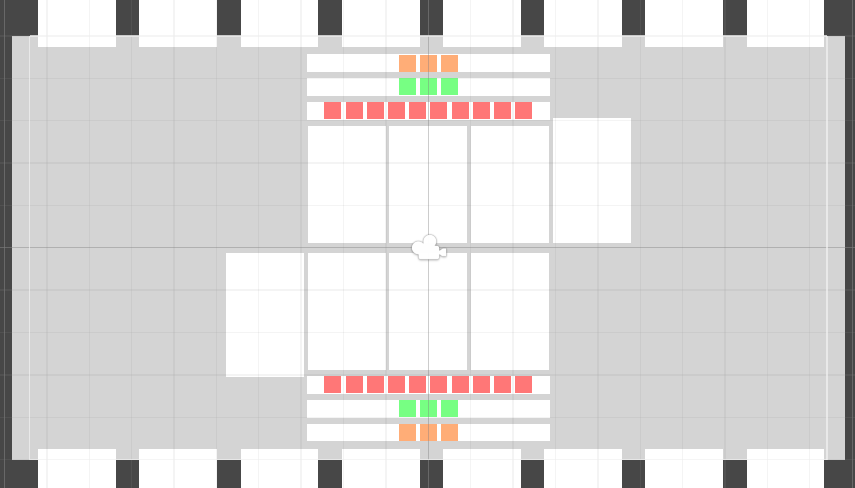
\includegraphics[width=400px,keepaspectratio]{images/proto.png}
        \label{Proto}
        \caption {Aréna prototípus}
    \hspace{1em}
\end{figure}

Ebben a fázisban a pálya már átlátható volt viszont még semmilyen funkció nem élt és az elrendezés kézzel történt. A későbbi verziókban történő változások ennek a ténynek tudhatóak be, mivel itt még nem rendereljük dinamikusan a képernyő elemeke ( az élet pontokat, akció- és reakció pontokat stb). Ez a későbbiekben Unity-n belül használható layoutok segítségével fogjuk megoldani.

\clearpage

\subsection{Első verzió}

\begin{figure}[h]
        \centering
        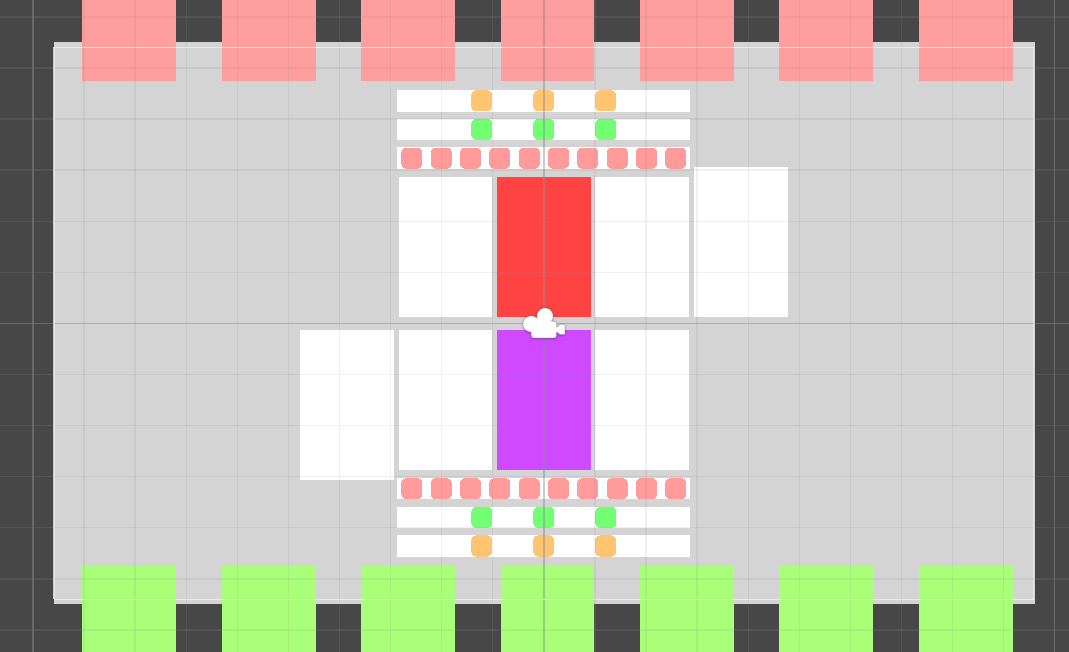
\includegraphics[width=400px,keepaspectratio]{images/Boardconcept.png}
        \label{ArenaLvl2}
        \caption {Aréna prefab-ekkel}
    \hspace{1em}
\end{figure}

Ebben a fázisban a kézzel elhelyezett elemeket átvették a layoutok és a prefabok. A már előbb említett layaoutok egy konzisztens elhelyezkedést garantálnak az elemeknek. Felmerülhet a kérdés hogy mik is azok a prefabok. A prefabok olyan játék objektumok amik le vannak mentve mint egy összeszerelt entitás. Megtudjuk határozni ennek a tulajdonságai és a rajta lép scripteket előre. Így mikor létre akarunk hozni egy játék objectumot akkor elég csak ezt a prefabot meghívni. A fenti ábrán látható: kártyák, élet pontok, akció pontok, és reakció pontok mind a játékos mind az ellenfél oldalán prefabokat használnak.


\clearpage

\subsection{Második Verzió}

A következő lépésben hozzá adtuk az End Turn gombot és a Karakter képét. Ezen felül a kézben lévő kártyákat generáljuk ahelyett hogy csak előre bele lennének helyezve a layoutba. A Felszerelés kártyák teszetlésének érdekében ideiglenesen bekerült egy extra kártya hely.

\begin{figure}[h]
        \centering
        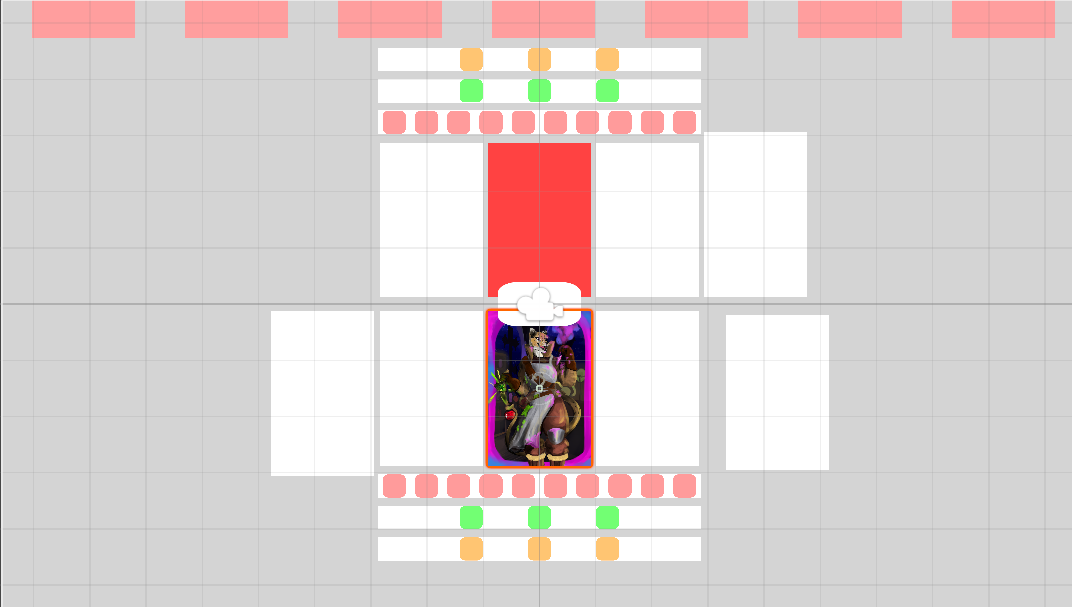
\includegraphics[width=400px,keepaspectratio]{images/board1.png}
        \label{ArenaLvl3_v1}
        \caption {Aréna futtatás előtt a kézzel berakott elemekkel}
    \hspace{1em}
\end{figure}
\begin{figure}[h]
        \centering
        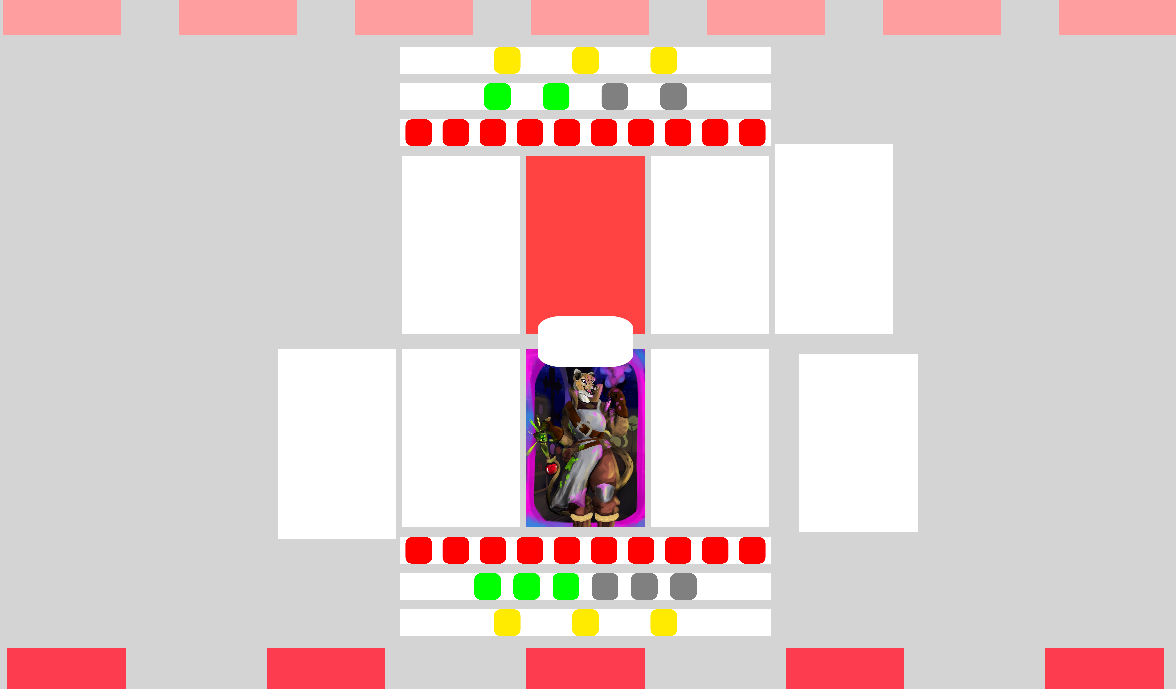
\includegraphics[width=400px,keepaspectratio]{images/board2.png}
        \label{ArenaLvl3_v2}
        \caption {Aréna futtatás után a generált elemekkel}
    \hspace{1em}
\end{figure}

\clearpage

\subsection{Végső Verzió}
Ez után az aréna végső stáduimba lépett. Az élet pontok át lettek formázba egy kicsit és a számuk meg lett növeltve 10->20. Az ideiglenes kártya hely ki lett véve. A játékos kártyáit mostmár a játékos paklija alapján, abból generálja a játék. Az élet csíkon a bal oldalra be lett helyezve egy mutató ami a pajzs értéket mutatja, a jobb oldalon pedig egy másik mutató ami pedig az élet pontokat mutatja. Ez az ellenfél oldalon is bekerült. Az End Turn gomb is kapott egy feliratot illetve zöld színű lett hogy jelezze hogy a játékos kezd.

\begin{figure}[h]
        \centering
        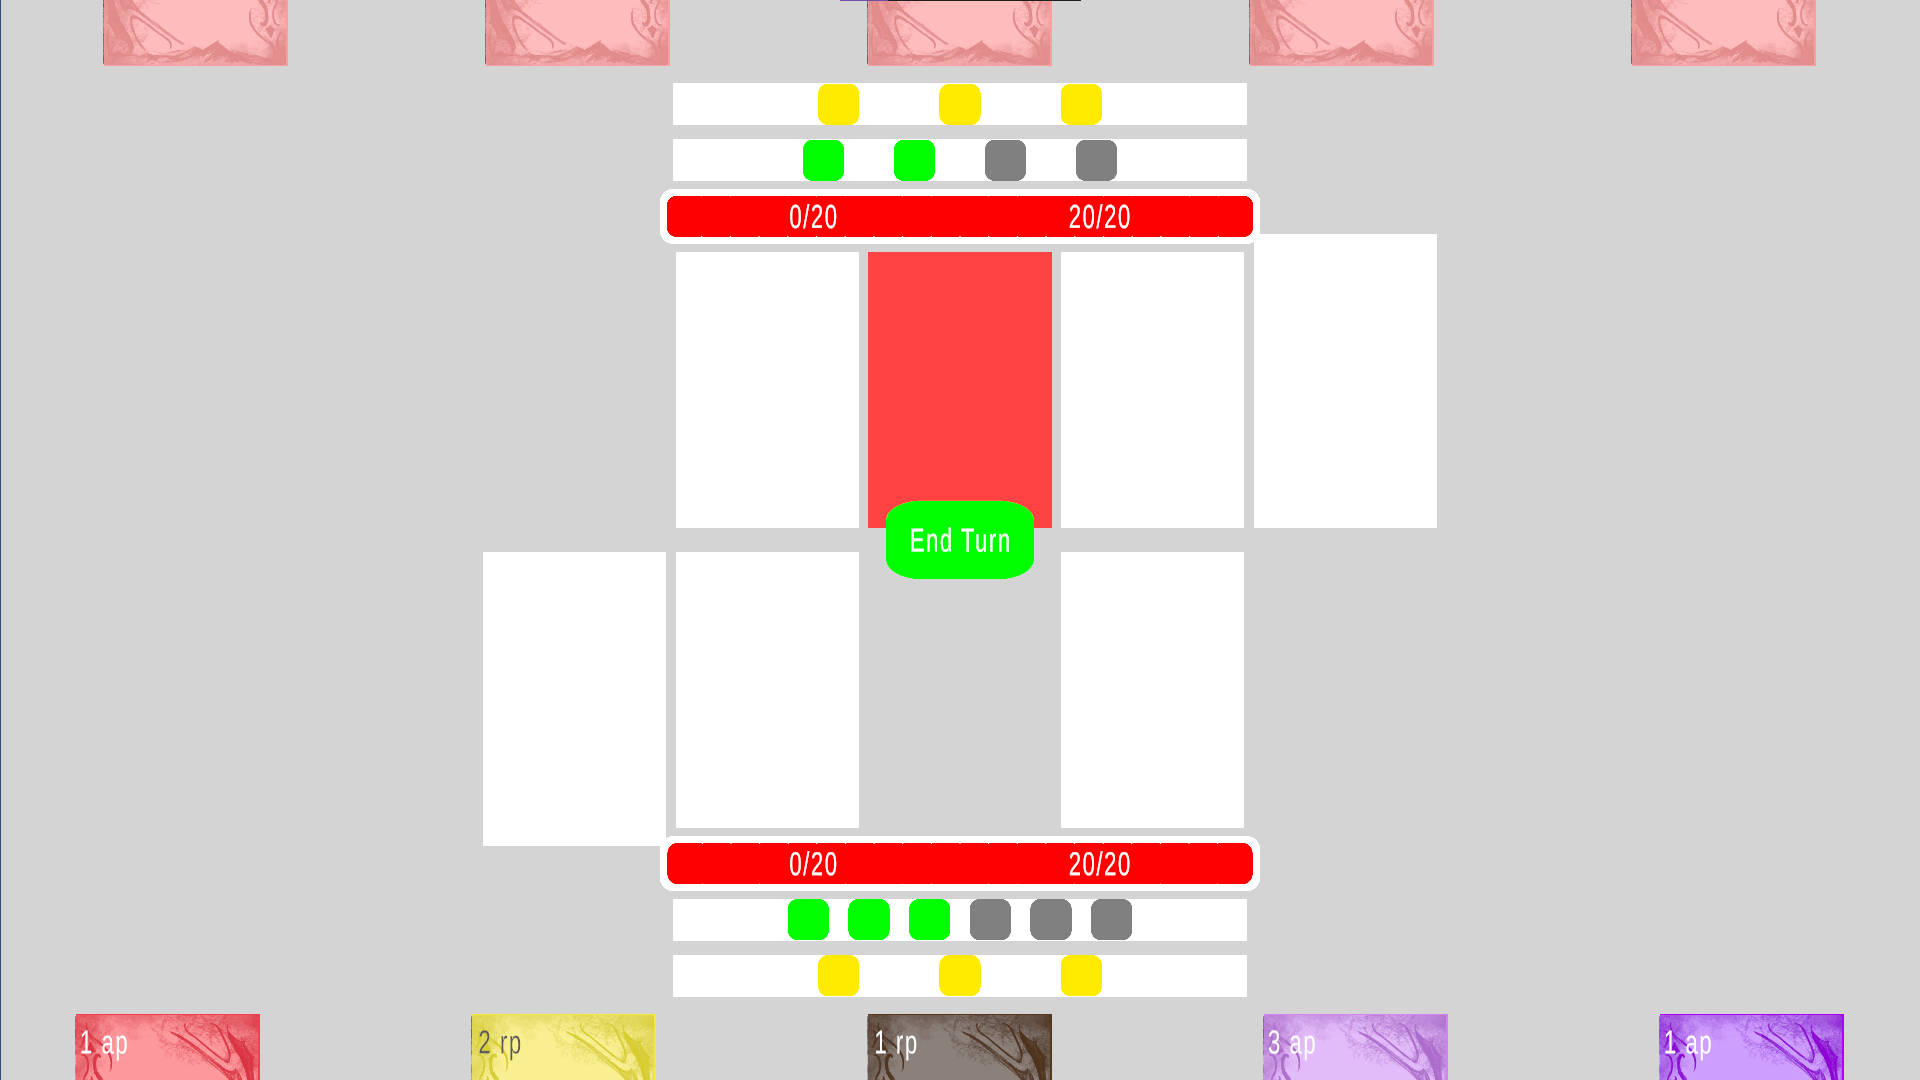
\includegraphics[width=400px,keepaspectratio]{images/image.png}
        \label{ArenaFinal}
        \caption {Aréna végső fázisban}
    \hspace{1em}
\end{figure}

Ez a verzió fogad minket amikor elkezdünk játszani.

\clearpage

\section{Kártya Húzás}
\subsection{Scriptable objects}
A karakterek információ (élet pontok, bónus sebzés, stb) egy-egy scriptable objectbe vannak letárolva. Ezek olyan játék objectumok amelyek információt tárolnak. Írthatóak és olvashatóak. Nagyon hasznosak mivel így van egy előre elkészített struktúra ami le tudja tárolni egy adott típusú objectum információit.
\\\
\begin{lstlisting}[language=CSharp,style=CSharpBase,caption={A Klass Scriptable Object kódja}]
using System.Collections;
using System.Collections.Generic;
using UnityEngine;

public enum Classes
{
    Warrior, Ranger, Necromancer,Paladin,Alchemist,Ninja,Druid,Mage
}

public enum WeaponTypes 
{
    Melee,Ranged,Magic,Summon
}

[CreateAssetMenu(menuName = "KlassData")]
public class ClassDataSo : ScriptableObject
{

    public int maxHp;
    public int currentHp;
    public int shield;
    public int maxAp;
    public int currentAp;
    public int apRegain;
    public int maxRap;
    public int currentRap;
    public int attackDmgBonus;
    public int spellDmgBonus;
    public Sprite sprite;
    public Classes characterKlass;
    public WeaponTypes weapon;
    public GameObject prefab;
    public List<CardDataSo> baseDeck;
    public List<CardDataSo> deck = new();
}
\end{lstlisting}

\clearpage

\subsection{A húzás működése}
Amikor a játékot elíndidjuk a karakter SO-jéból (Scriptable Object) kivesszük az alap paklit. Ezt behejezzük a játékon belül használt pakliba. Ez a pakli fog változni amikor kártyát húznuk illetve amikor kártyát vissza teszünk. A pakli egy lista ami a benne lévő kártyák információját tárolja. A kártyák egy másik SO-ba vannak letárolva. Kártya húzáskor ezt a kártya SO-t inicializáljuk az az egy fizikai játék objectumként hozunk létre.
Még mielőtt a kártya létrejöhetne meg kell nézzük hogy belefér e a játékos kezébe. Ha nem akkor a húzás nem történik meg. Ha igen akkor a kártyának a vizuális elemeit frissítjük (Ára, neve, típusa, stb). Miután ez megtörtént létrehozzuk az objectumot és megadjuk neki hogy melyik kártya SO hozta létre. Ez a fizikai objectum lesz majd kijátszható a játékos által.
\\\
\begin{lstlisting}[language=CSharp,style=CSharpBase,caption={A kártya kézbe helyezése}]
public void PutCardInHand()
{
    if (deck.Count == 0 || hand.childCount >= 10)
    {
        return;
    }
    var data = deck[0];
    if (data.isActionCost)
    {
        data.prefab.transform.Find("price").GetComponent<TextMeshPro>().text = 
        string.Concat(data.cost) + " ap";
    }
    else
    {
        data.prefab.transform.Find("price").GetComponent<TextMeshPro>().text = 
        string.Concat(data.cost) + " rp";
    }
    data.prefab.transform.Find("Desc").GetComponent<TextMeshPro>().text =
    string.Concat(data.description);
    
    data.prefab.transform.Find("dmg").GetComponent<TextMeshPro>().text = 
    string.Concat(data.dmg);
    
    data.prefab.transform.Find("Type").GetComponent<TextMeshPro>().text = 
    string.Concat(data.cardType);
    
    var card = Instantiate(data.prefab, hand);
    card.GetComponent<Card>().data = data;
    deck.Remove(deck[0]);
}
\end{lstlisting}
\clearpage
\section{Kártya Kijátszás}
A kártyák kijátszása a Unity ActionHandler system-ével működik. Ez az event system úgy működik hogy van egy event stack. Erre a stackre iratkoznak fel az egyes metódusok. És amikor invoke-oljuk ezt a stacket az összes metódus meghívódik ami feliratkozott. Ezek a metódusok nem törlődnek amikor a stack meghívásra kerül.
\\\
\begin{lstlisting}[language=CSharp,style=CSharpBase,caption={Event kezelő}]
using System.Collections;
using System.Collections.Generic;
using UnityEngine;

public class CardAction : MonoBehaviour
{
    public delegate void ActionHandler();
    public ActionHandler onCardPlayed;
    CardDataSo data;
    void Start()
    {
        data = GetComponent<Card>().data;
    }

    public void PlayCard() 
    {
        onCardPlayed?.Invoke();
        if (GameManager.instance.heroData.currentAp >
                                GameManager.instance.heroData.maxAp 
            || GameManager.instance.heroData.currentHp >
                                GameManager.instance.heroData.maxHp)
        {
            GameManager.instance.heroData.SetToMax();
        }
    }  
}
\end{lstlisting}

\section{Mesterséges inteligencia}
Annak köszönhetően hogy a játék egyszemélyes szükség van egy ellenfélre aki ellen a játékos tud játszani. Az ellenség egy egyszerű mesterséges inteligenciát alkalmaz. Képes támadni, gyógyítani magán, pajzsot adni magának, felszerelést lehelyezni illetve 5 lappal kezdi mindegy egyes körét. 

Ezeken felül hogy a játék egyre nehezedjen ahogy haladunk előre az ellenfél minden új csata folyamán kap 5 plusz életpontot, minden 3. kör alkalmával pedig plusz 1 akció- és reakció pontot, plusz egy akció pontot nyer vissza körönként és plusz 1 kártyát kap körönként.

%Diagrammok és folyamat ábrák
%másjátékokkal valú összahasonlítás (összehasonlító táblázat)
%
\chapter{Összefoglalás}

Hasonló szerepe van, mint a bevezetésnek.
Itt már múltidőben lehet beszélni.
A szerző saját meglátása szerint kell összegezni és értékelni a dolgozat fontosabb eredményeit.
Meg lehet benne említeni, hogy mi az ami jobban, mi az ami kevésbé jobban sikerült a tervezettnél.
El lehet benne mondani, hogy milyen további tervek, fejlesztési lehetőségek vannak még a témával kapcsolatban.


%biblatex verzió
%a bibintoc heading stílussal megjelenik a tartalomjegyzékben, title-lel a megjelenő címsor szövege módosítható
\printbibliography[heading=bibintoc,%
title=Források]
%sima bibtex verzió
%\bibliographystyle{plain}
%\bibliography{dolgozat.bib}

\pagestyle{empty}

\section*{CD Használati útmutató}

Ennek a címe lehet például \textit{A mellékelt CD tartalma} vagy \textit{Adathordozó használati útmutató} is.

Ez jellemzően csak egy fél-egy oldalas leírás.
Arra szolgál, hogy ha valaki kézhez kapja a szakdolgozathoz tartozó CD-t, akkor tudja, hogy mi hol van rajta.
Jellemzően elég csak felsorolni, hogy milyen jegyzékek vannak, és azokban mi található.
Az elkészített programok telepítéséhez, futtatásához tartozó instrukciók kerülhetnek ide.

A CD lemezre mindenképpen rá kell tenni
\begin{itemize}
\item a dolgozatot egy \texttt{dolgozat.pdf} fájl formájában,
\item a LaTeX forráskódját a dolgozatnak,
\item az elkészített programot, fontosabb futási eredményeket (például ha kép a kimenet),
\item egy útmutatót a CD használatához (ami lehet ez a fejezet külön PDF-be vagy MarkDown fájlként kimentve).
\end{itemize}


\end{document}
